\chapter{Specific Requirements}

\section{External Interface Requirements}

\subsection{User Interfaces}

In this section we describe and present a possible mock-up for the application, following the order of events proposed in the sequence diagrams.\\

At the launch of the application the user has to insert the credentials in the Log In page~\ref{fig:LogInMockup}. In case of new user, he can click on a button to open the Sign Up page~\ref{fig:SignUpMockup}, to create a new account.

% screenshots here
\begin{figure}[H]
	\centering     %%% not \center
	\subfigure[Log In page.]{\label{fig:LogInMockup}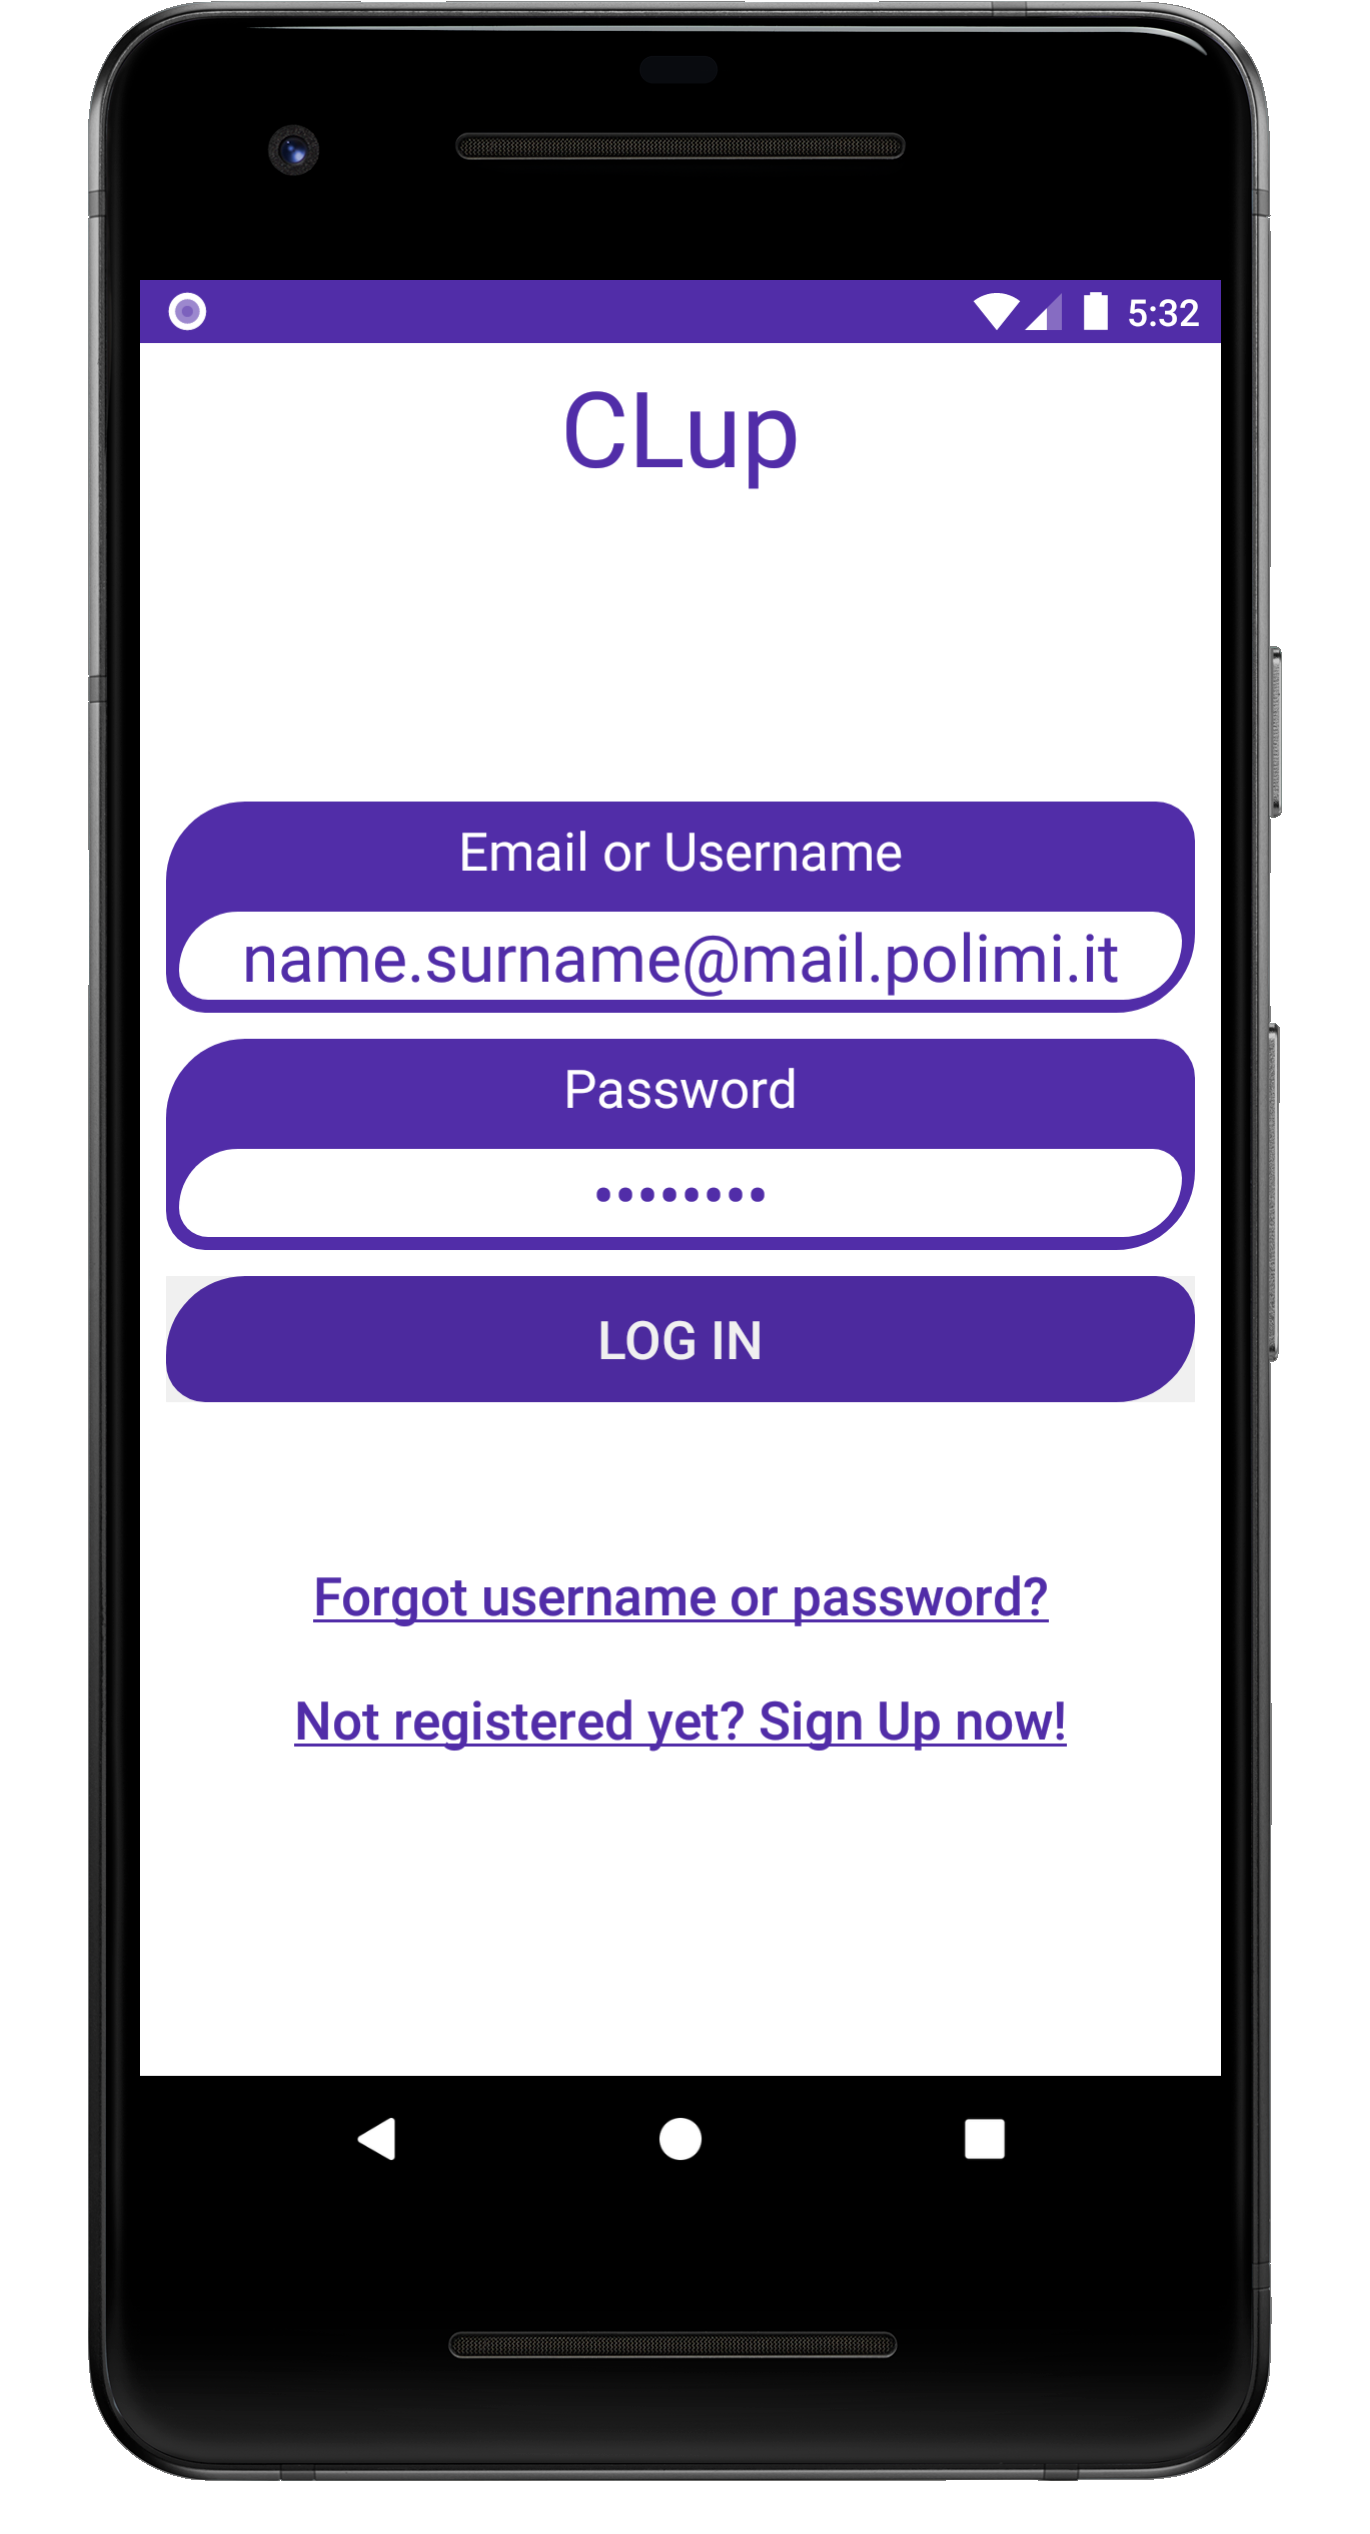
\includegraphics[width=0.4\textwidth]{images/log_in.png}}
	\subfigure[Sign Up page.]{\label{fig:SignUpMockup}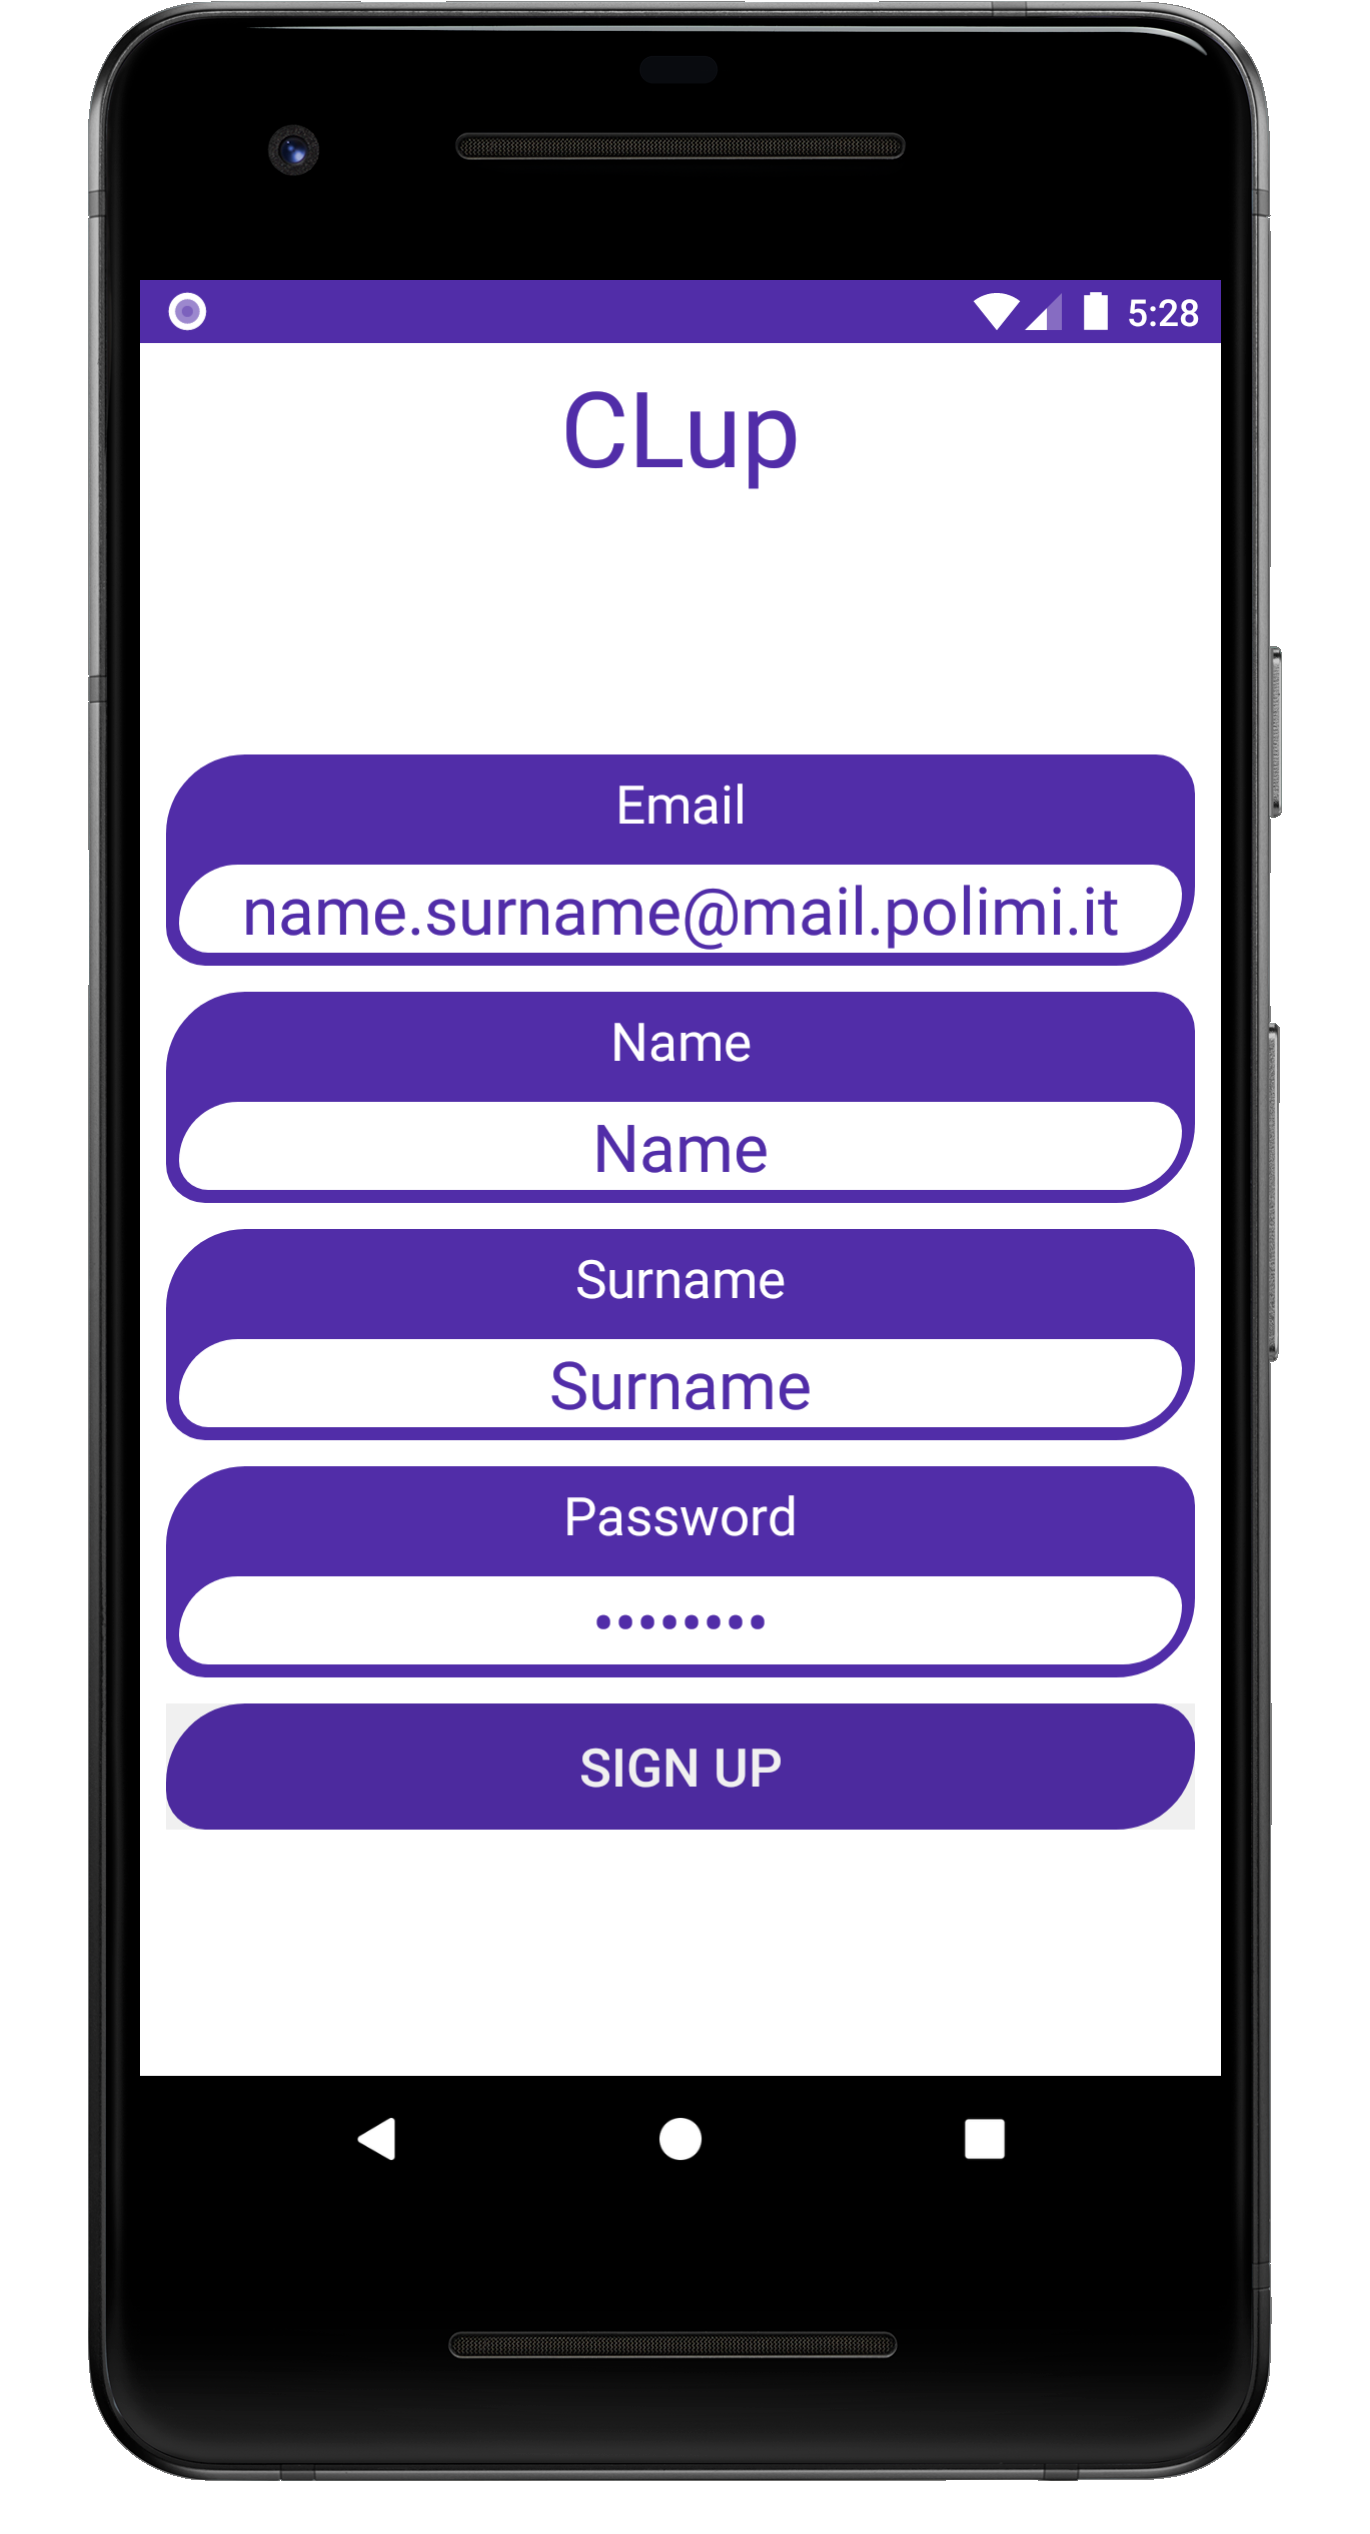
\includegraphics[width=0.4\textwidth]{images/sign_up.png}}
	\caption{Example of Log In and Sign Up pages.}
\end{figure}

Once the login has been completed successfully, the user is redirected to the Home page~\ref{fig:HomeMockup}.
In particular, the reported figure shows the Home page for the customer account with all the functionalities. The application, knowing the type of account, is able to show different buttons. For example, in case of physical spot account, the application will display only the Lining Up button, hiding the others. In case of store manager account, there will be displayed only buttons to control the queue and to analyze the statistics. 

\begin{figure}[H]
	\centering
	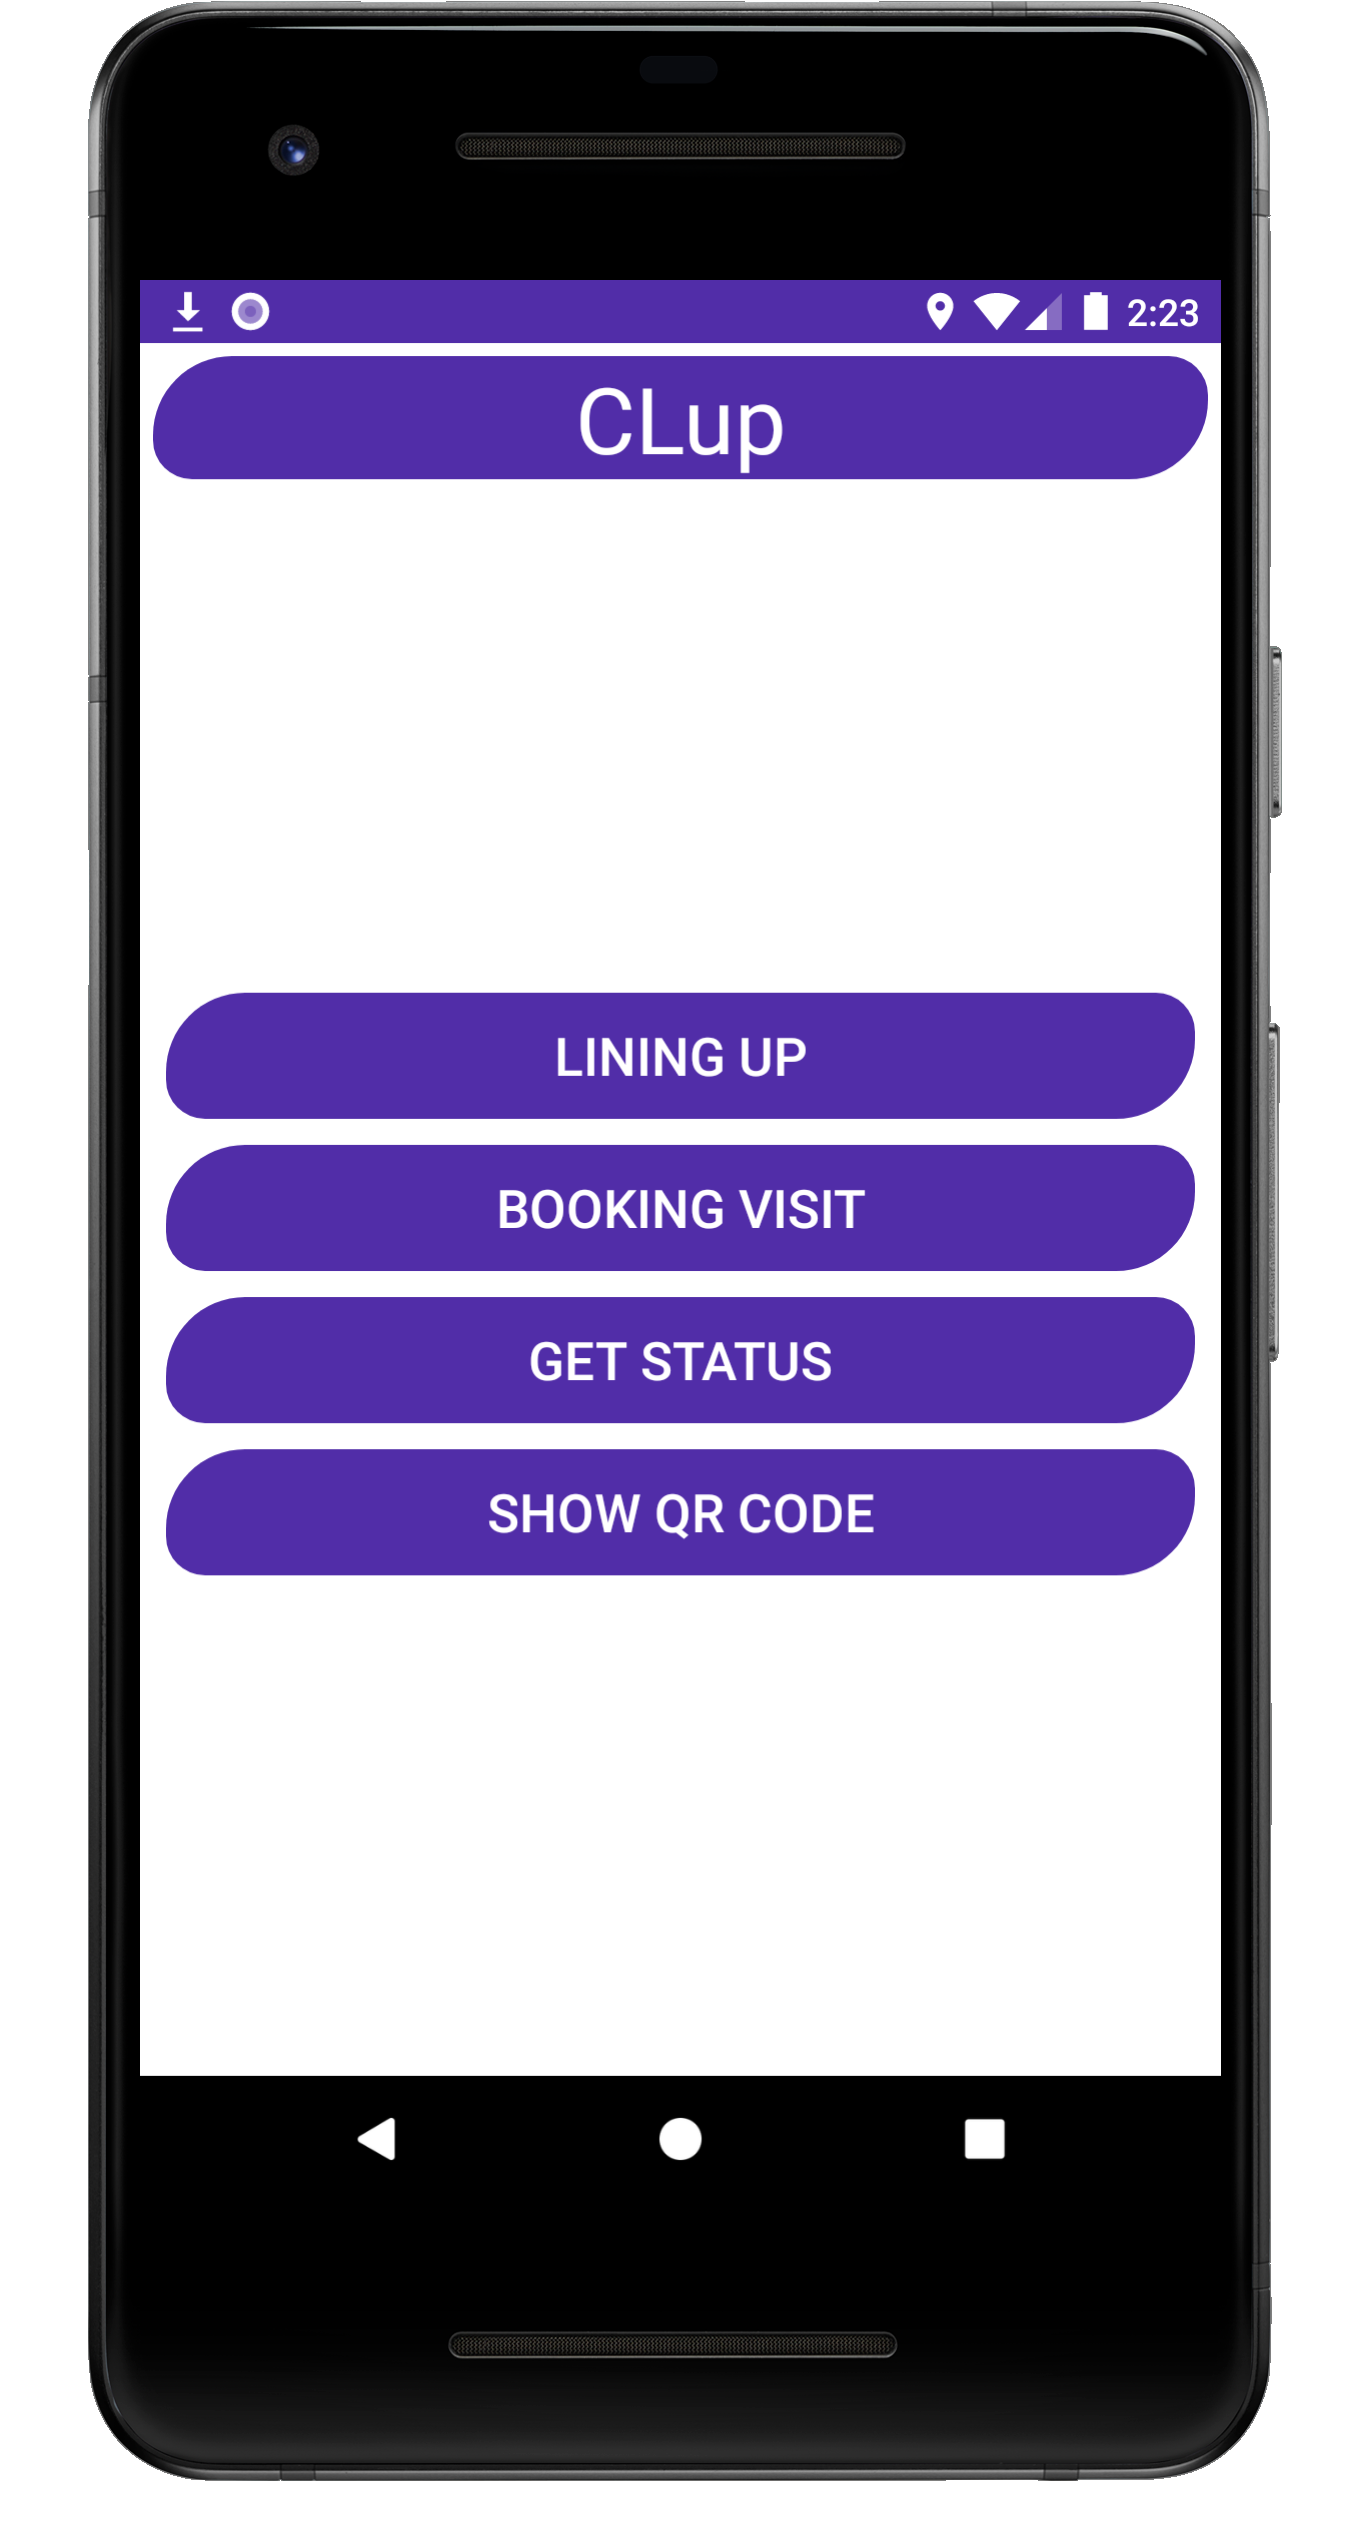
\includegraphics[width=0.35\textwidth]{images/home.png}
	\caption{Home page.}
	\label{fig:HomeMockup}
\end{figure}

If a customer wants to line up, or book a visit, he can click on the corresponding button, in this way the application will show the form to insert the requested parameters~\ref{fig:LiningBookingMockup}.
In the mock-up we show how the user can choose the store, the time slot and, in case of booking, the category of grocery, by expanding the drop down menu.

\begin{figure}[H]
	\centering     %%% not \center
	\subfigure[Lining Up page.]{\label{fig:LiningUpMockup}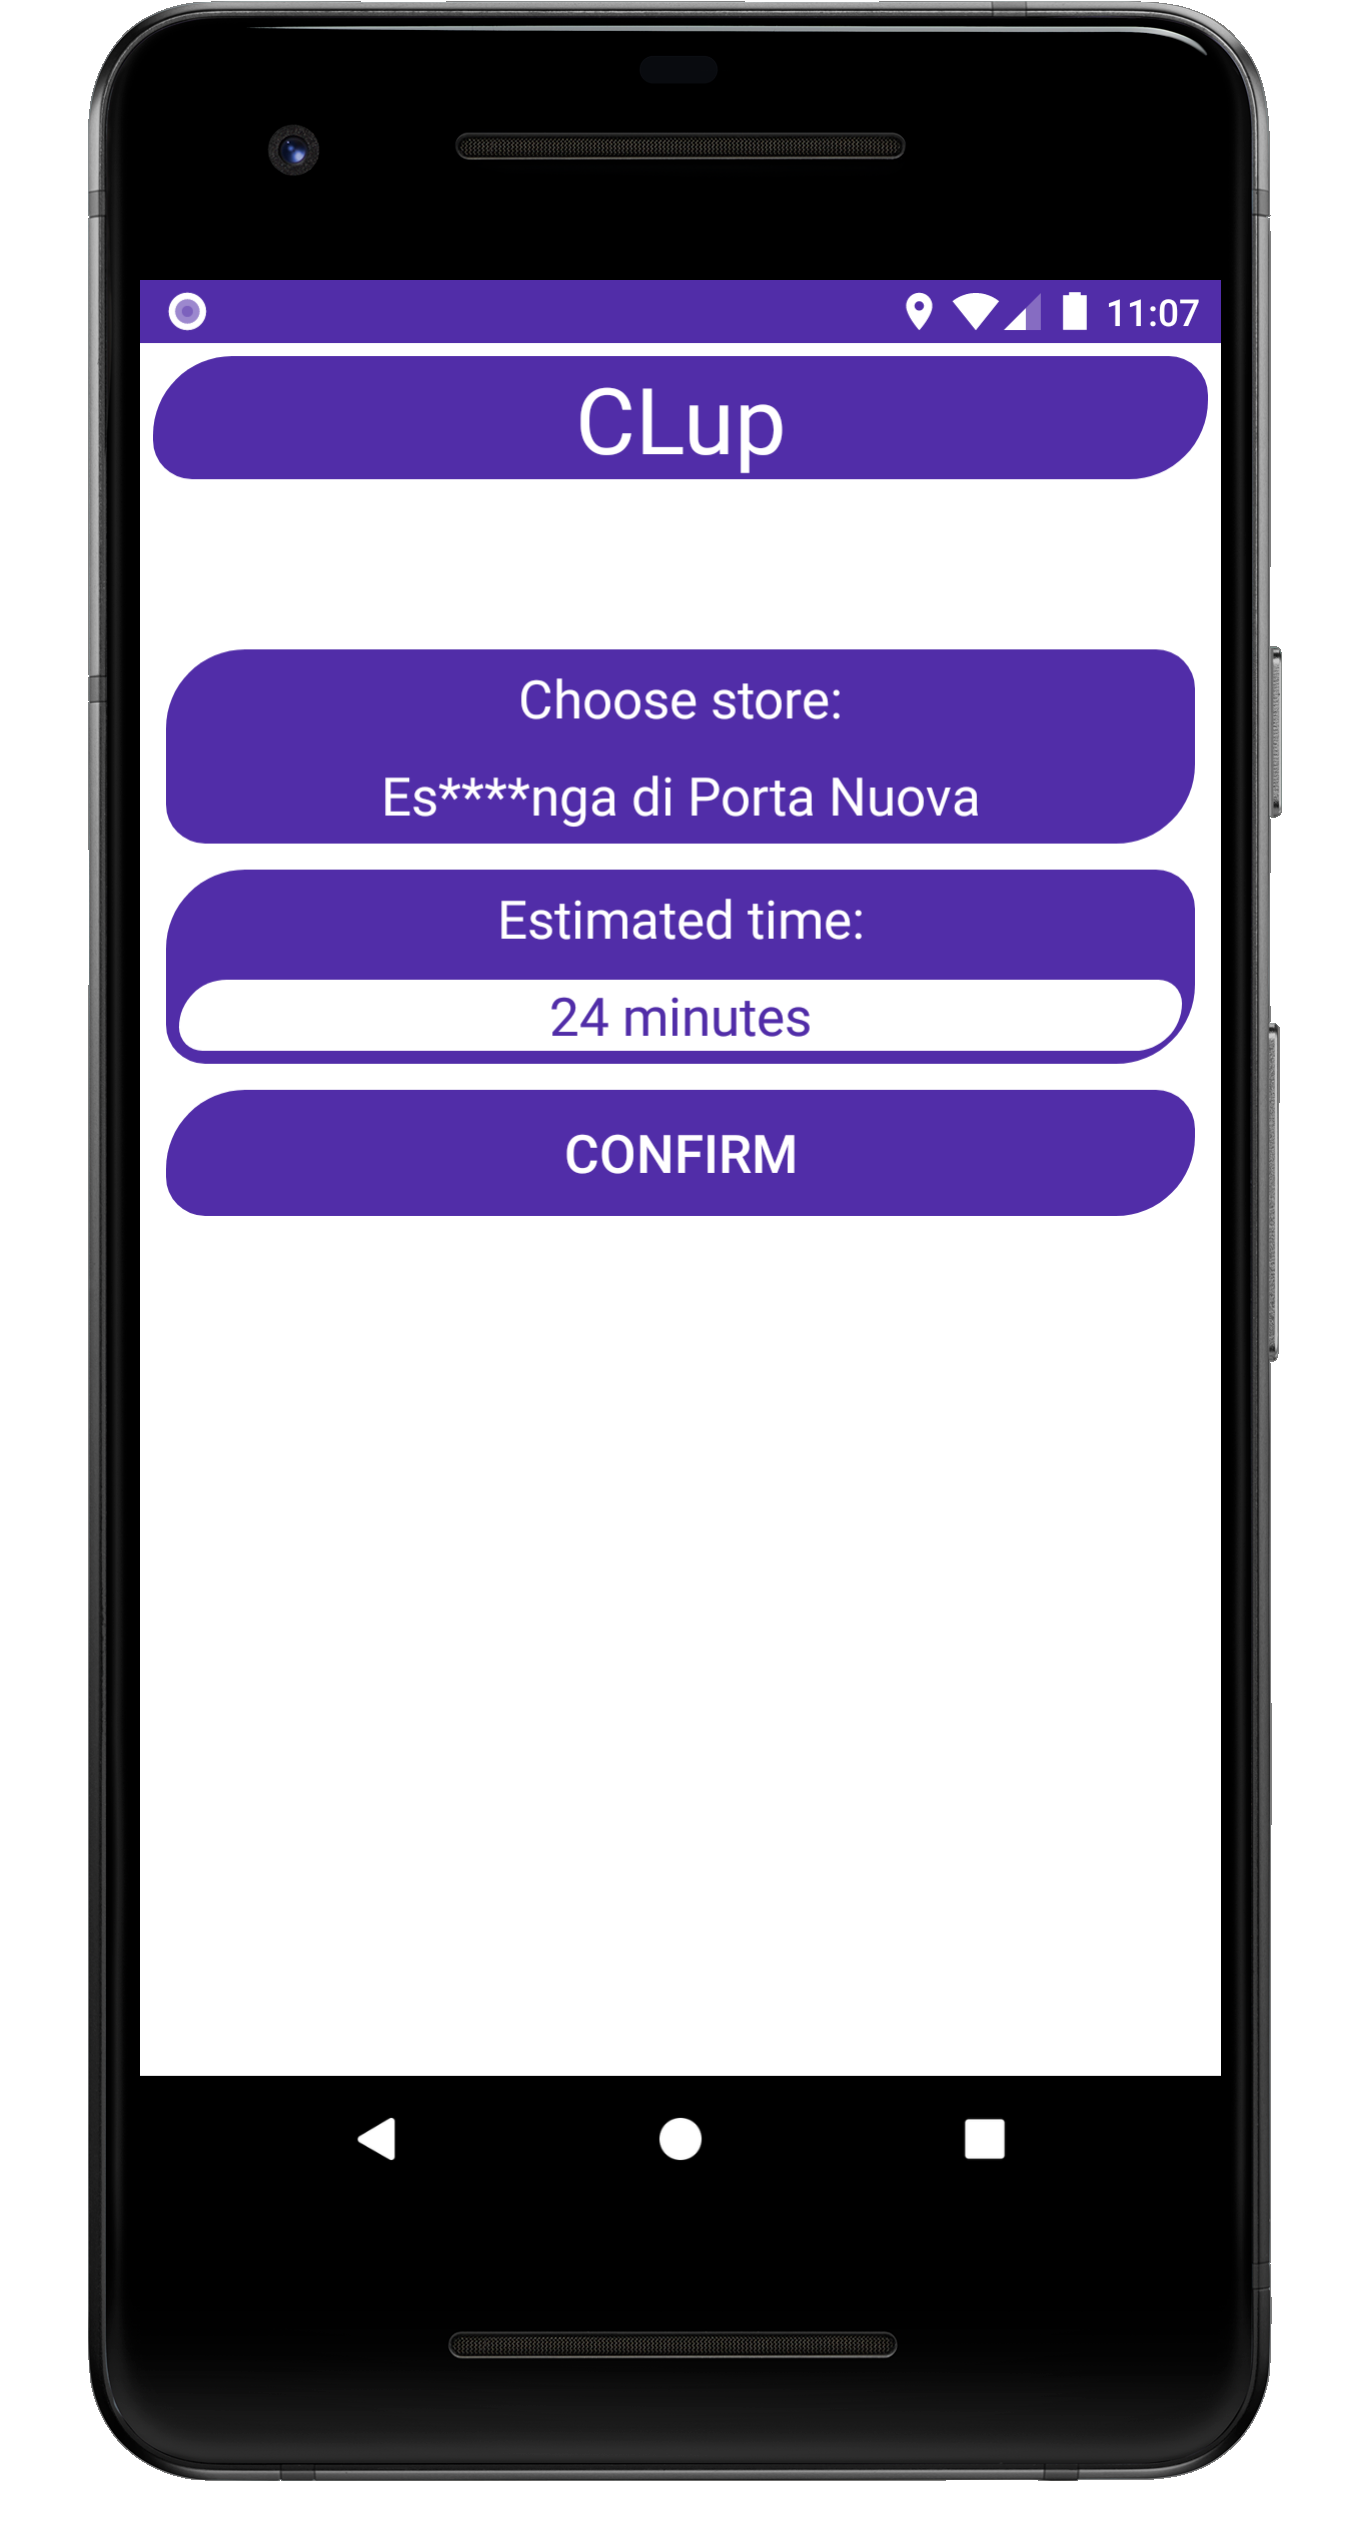
\includegraphics[width=0.4\textwidth]{images/lining_up_01.png}}
	\subfigure[Booking Visit page.]{\label{fig:BookingVisitMockup}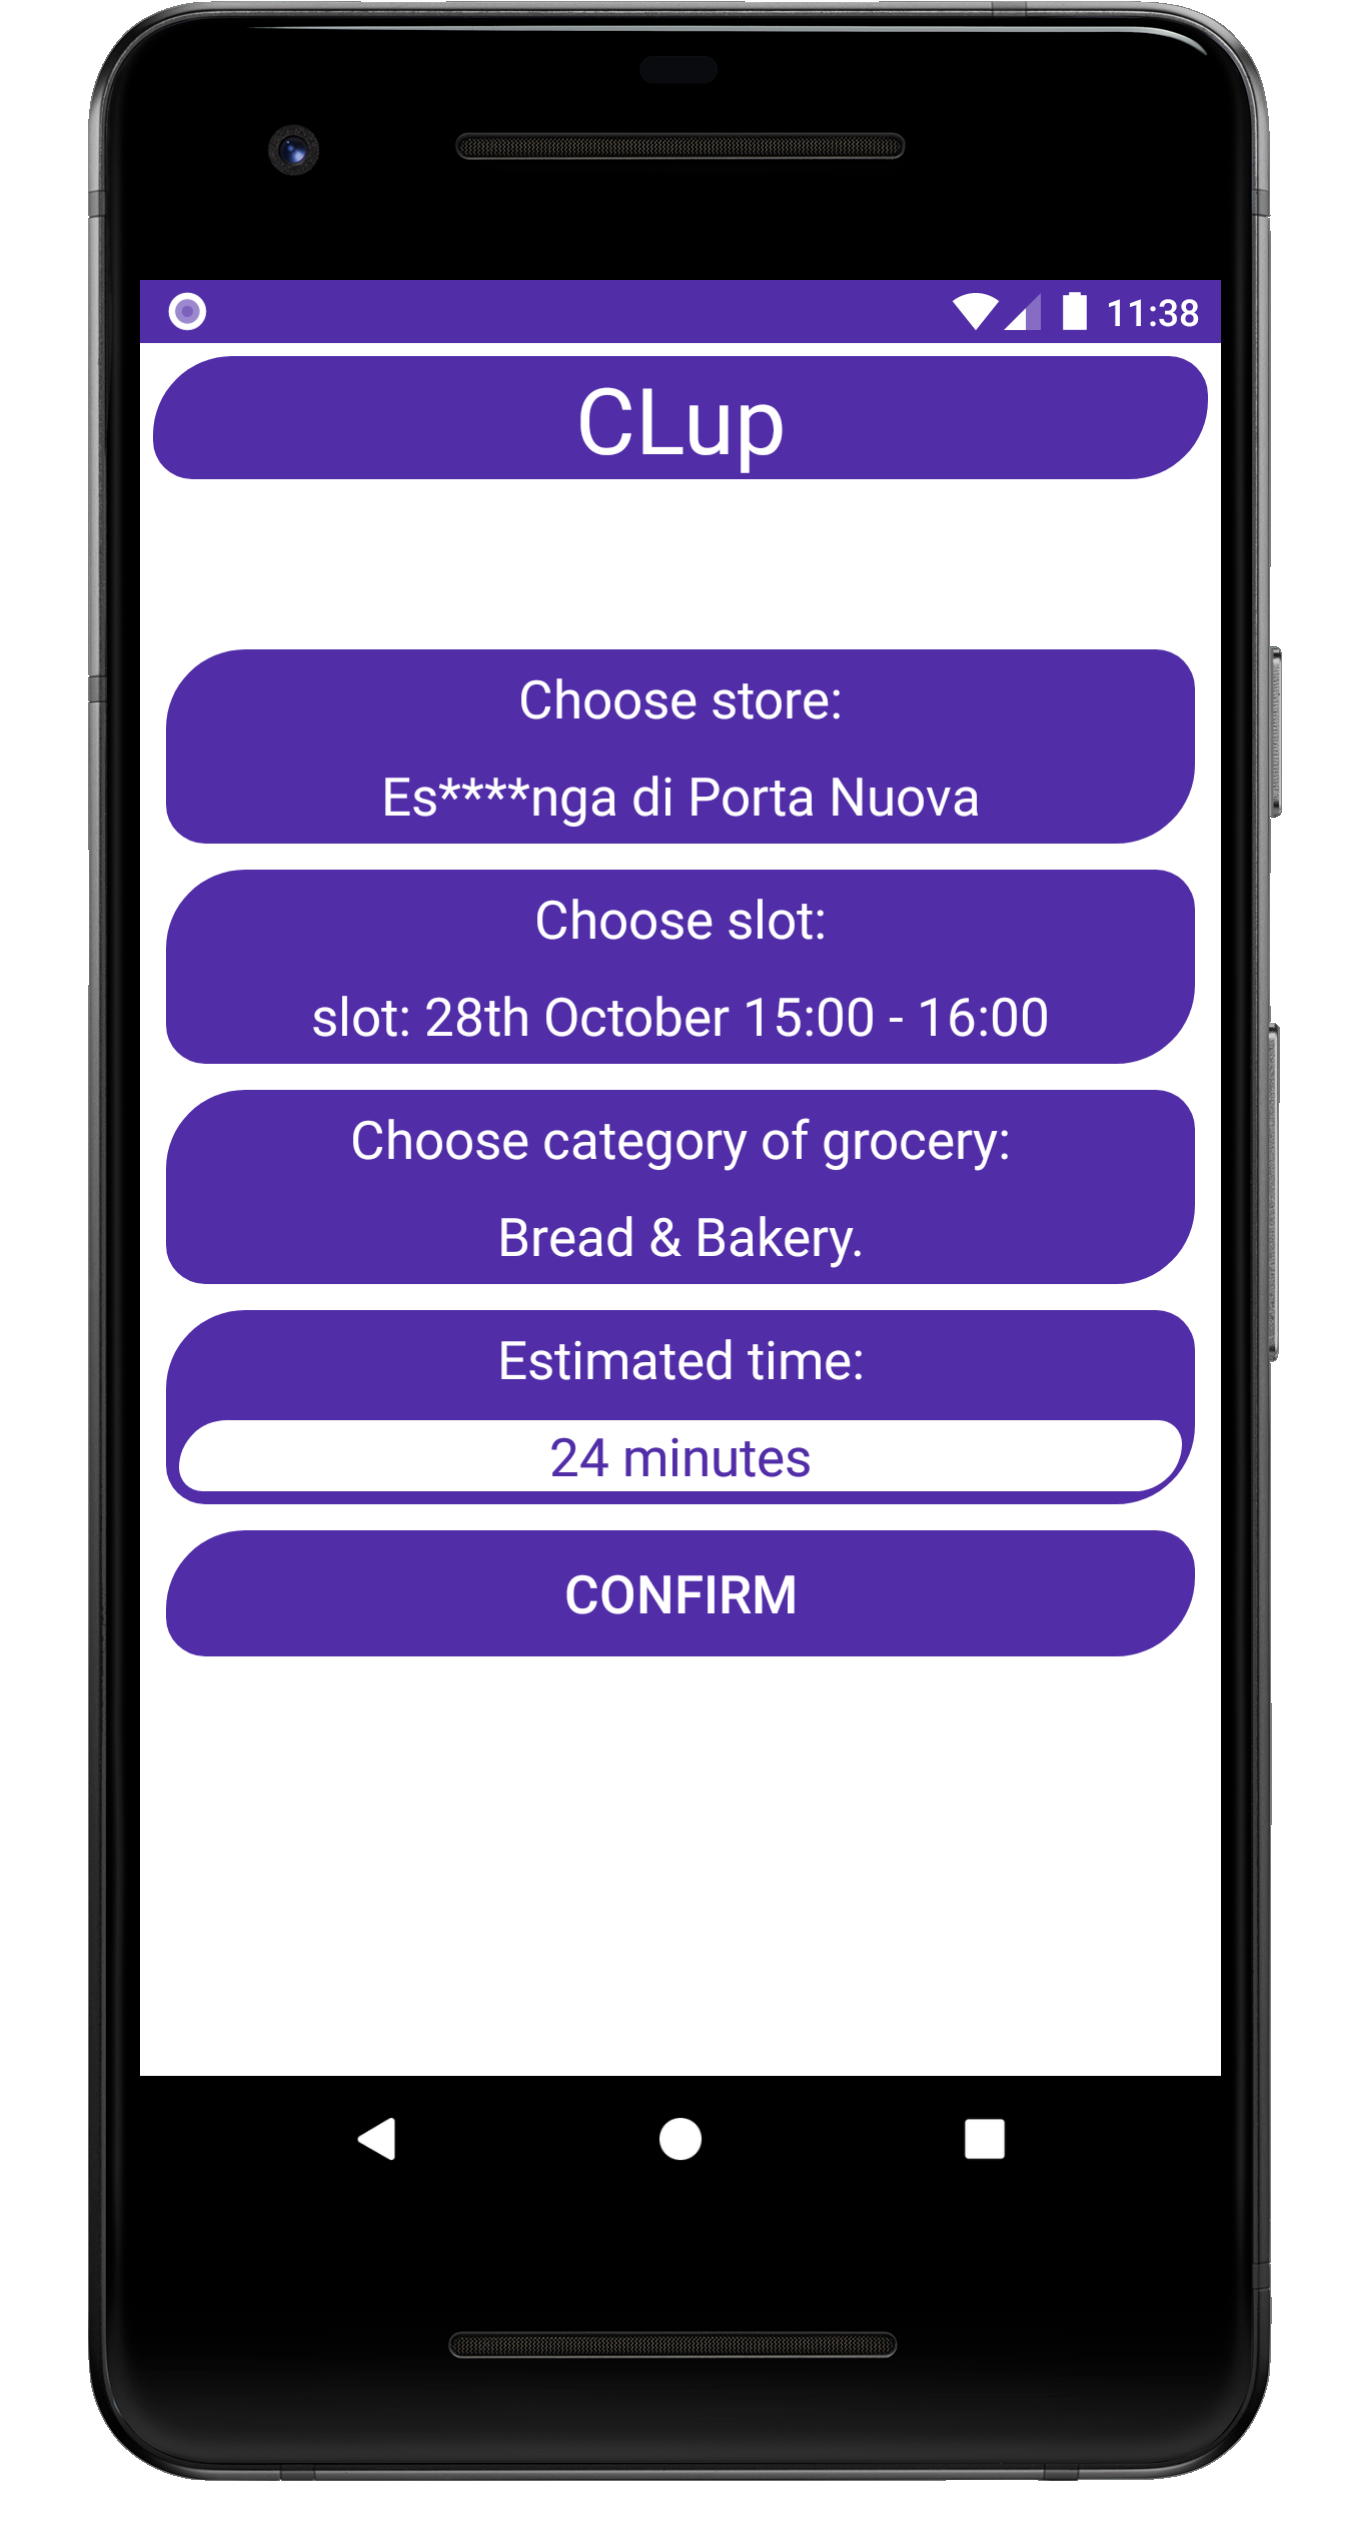
\includegraphics[width=0.4\textwidth]{images/booking_visit_01.png}}
	
	\subfigure[Lining Up page with expanded spinner.]{\label{fig:LiningUp2Mockup}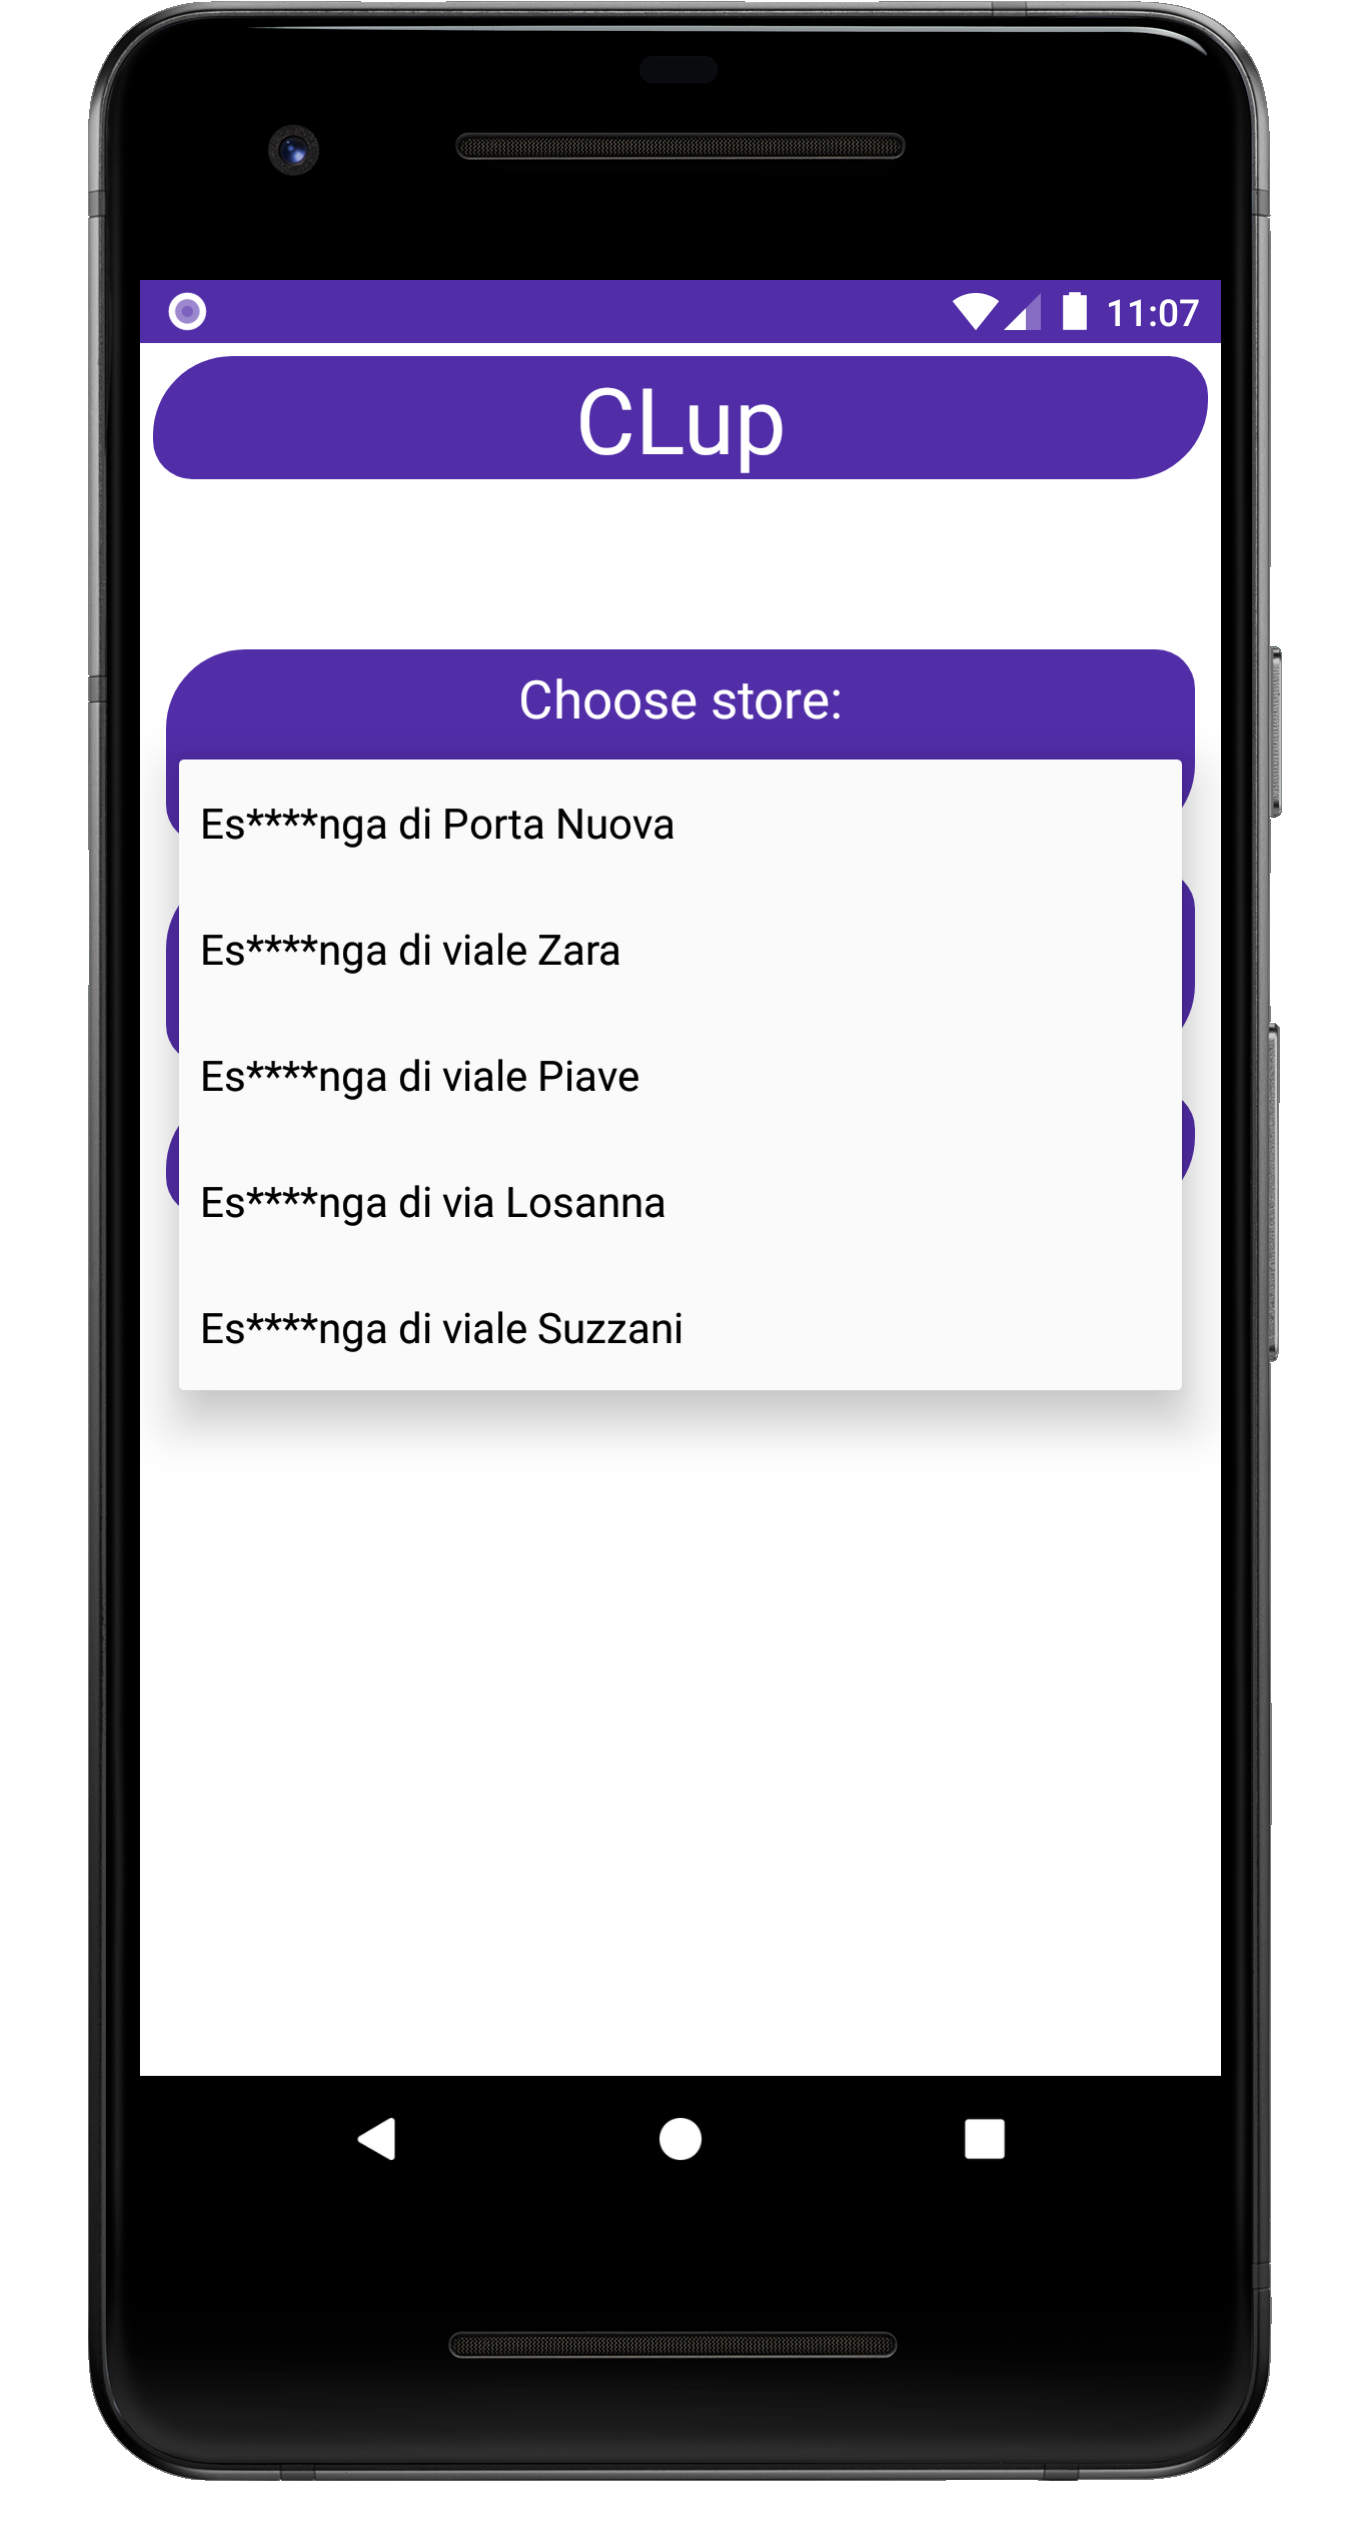
\includegraphics[width=0.4\textwidth]{images/lining_up_02.png}}
	\subfigure[Booking Visit page with expanded spinner.]{\label{fig:BookingVisit2Mockup}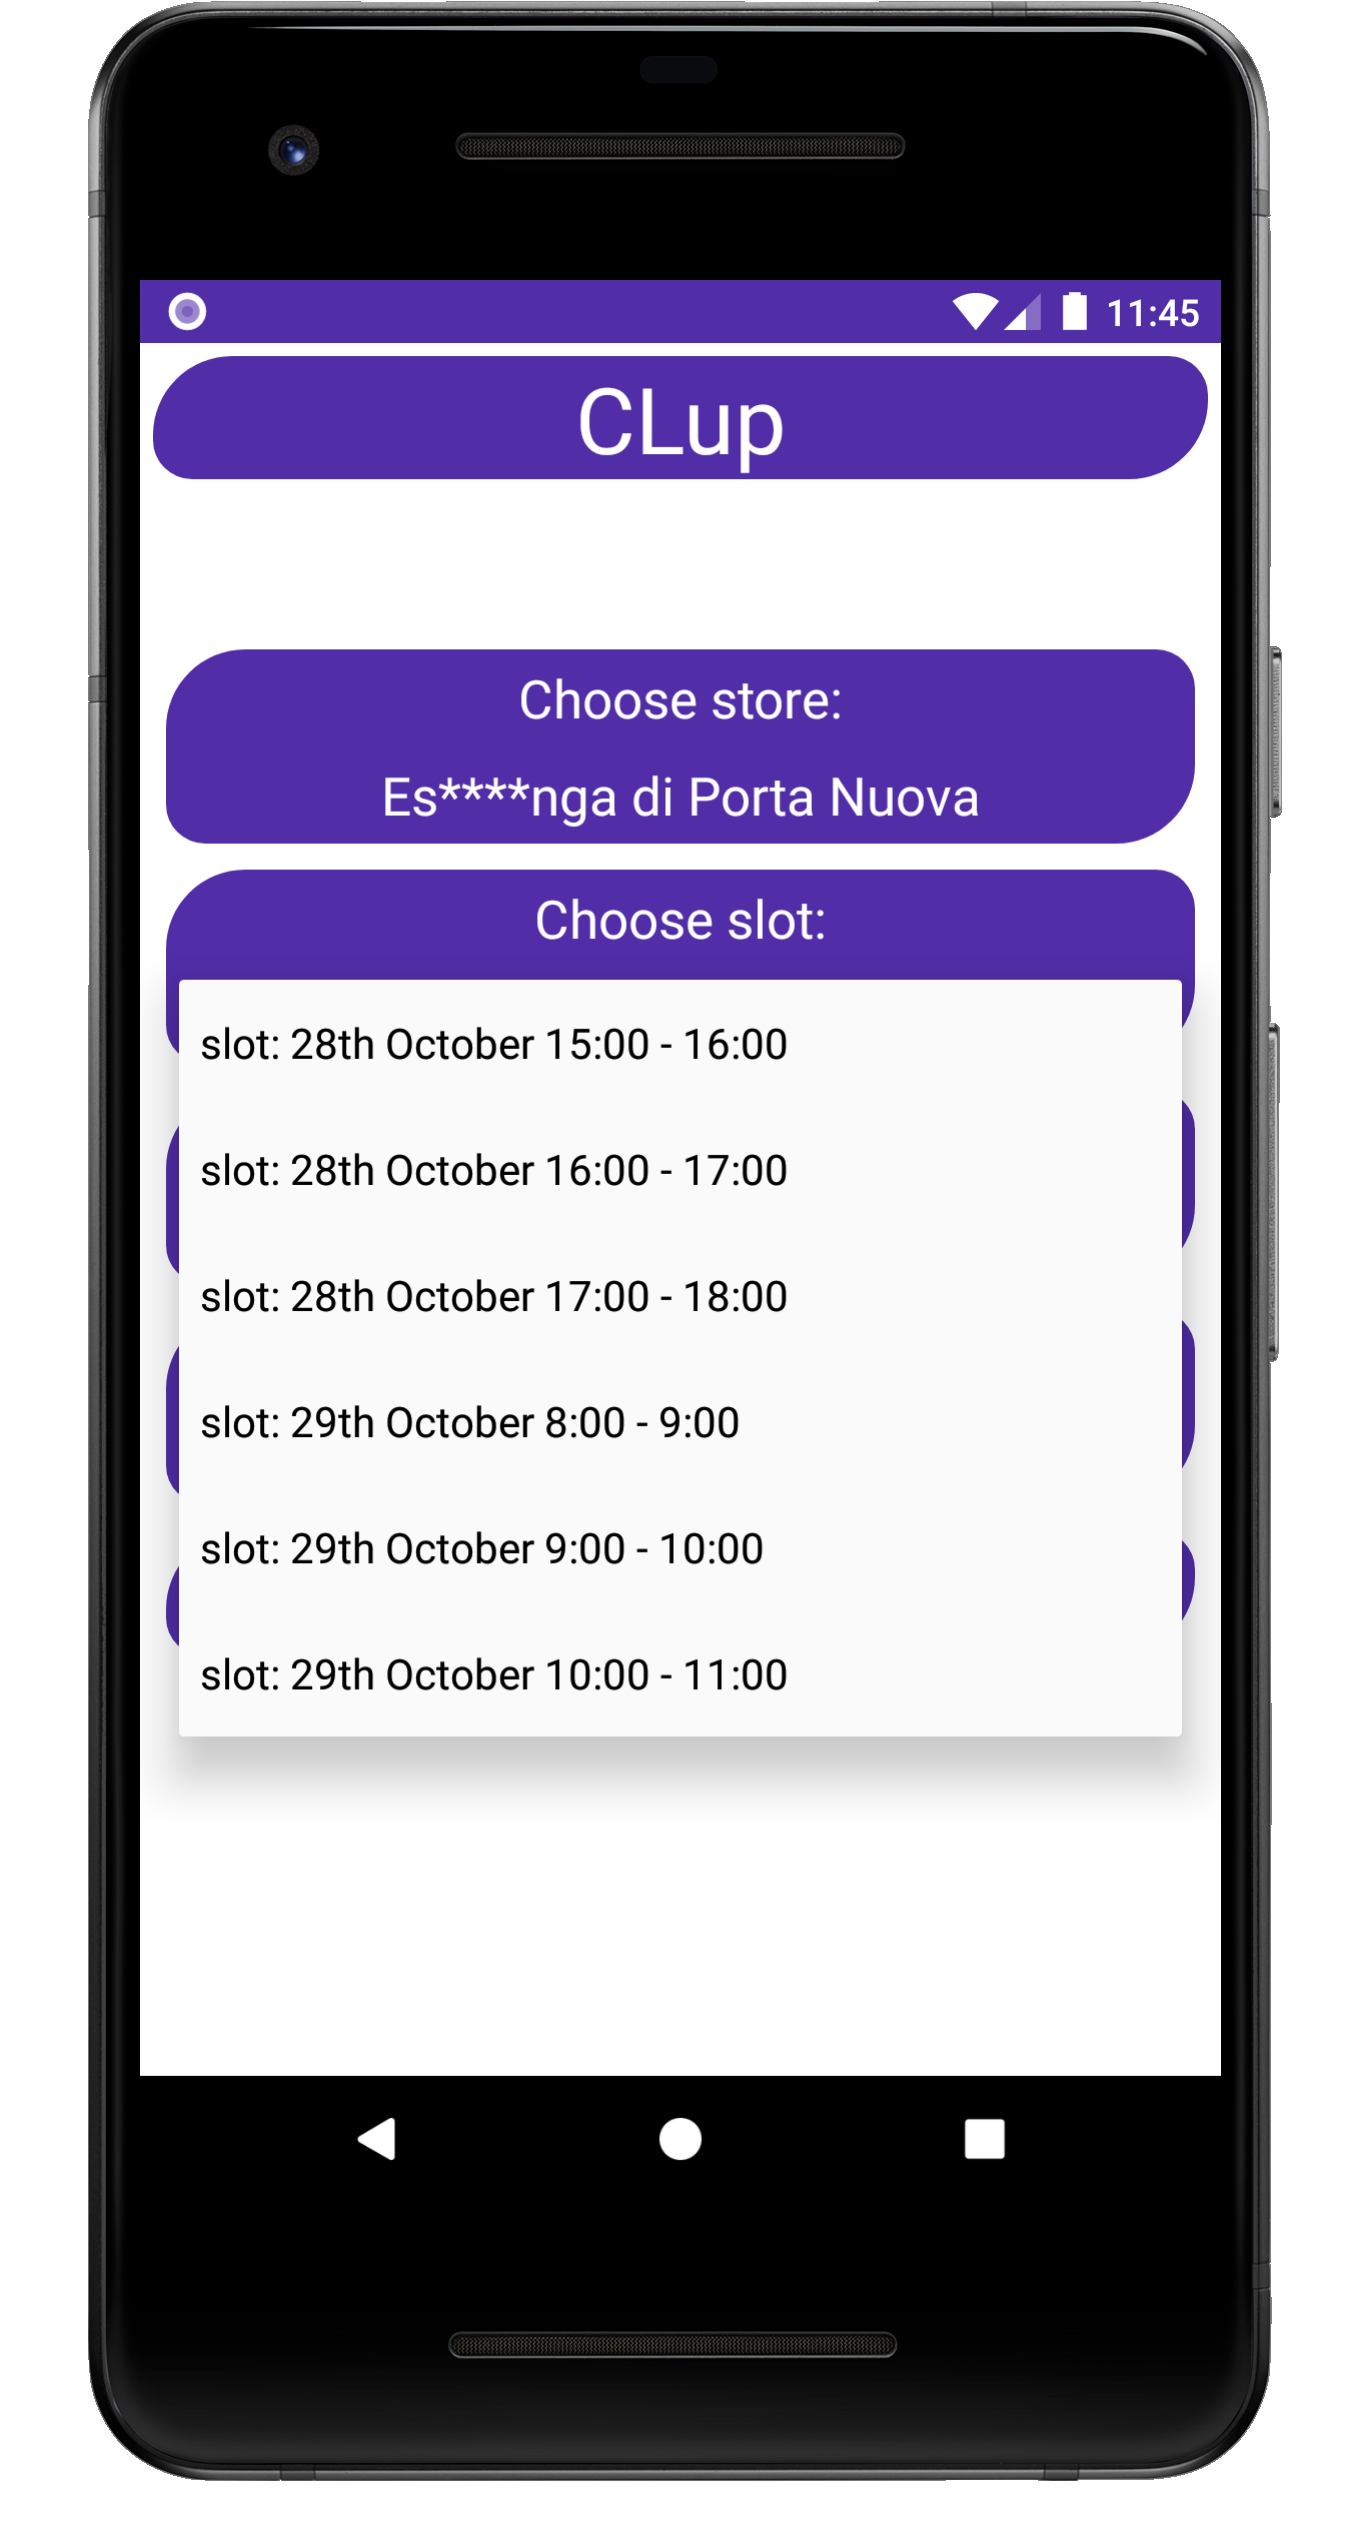
\includegraphics[width=0.4\textwidth]{images/booking_visit_02.png}}
	\caption{Example of Lining Up and Booking Visit pages.}
	\label{fig:LiningBookingMockup}
\end{figure}

The application provides the possibility to check the queue status by clicking on the Get Status button and to watch the QR code by clicking on the relative button.
These buttons aren't visible from the Home page until the user performs a lining up, or booking a visit, operation.
If visible, the users will be able to see the interfaces: \ref{fig:GetStatusMockup}, \ref{fig:ShowQRMockup}.

\begin{figure}[H]
	\centering     %%% not \center
	\subfigure[Get Status page.]{\label{fig:GetStatusMockup}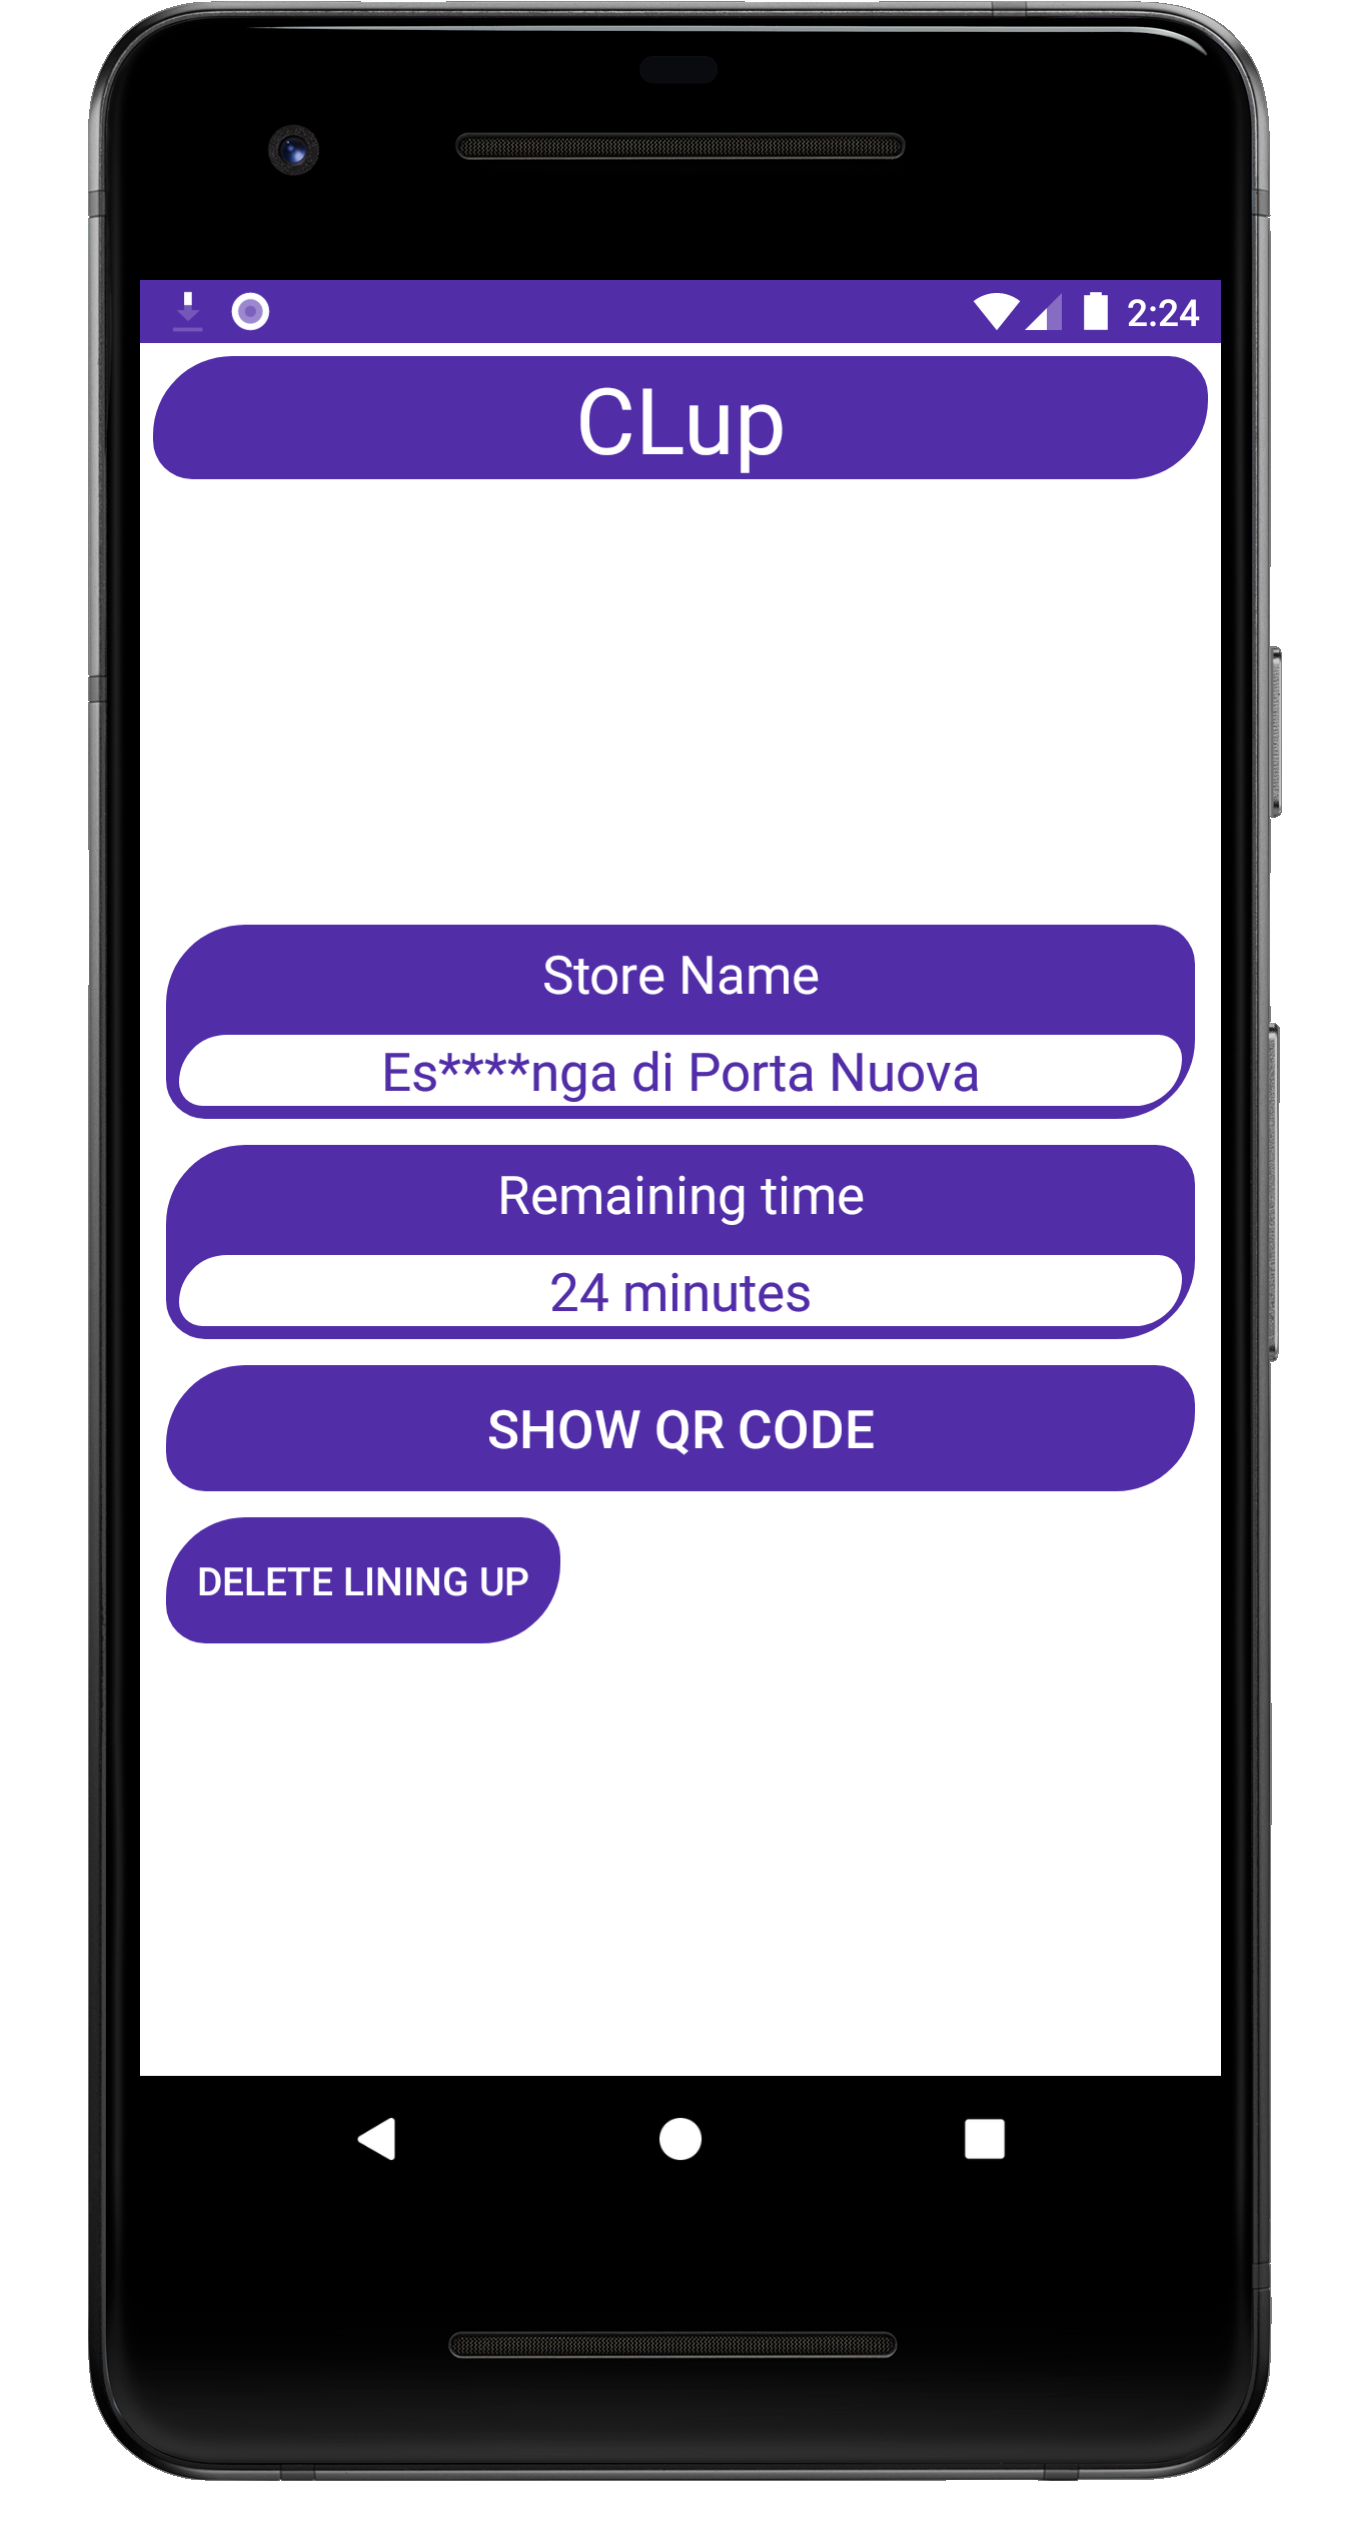
\includegraphics[width=0.4\textwidth]{images/get_status.png}}
	\subfigure[Show QR code page.]{\label{fig:ShowQRMockup}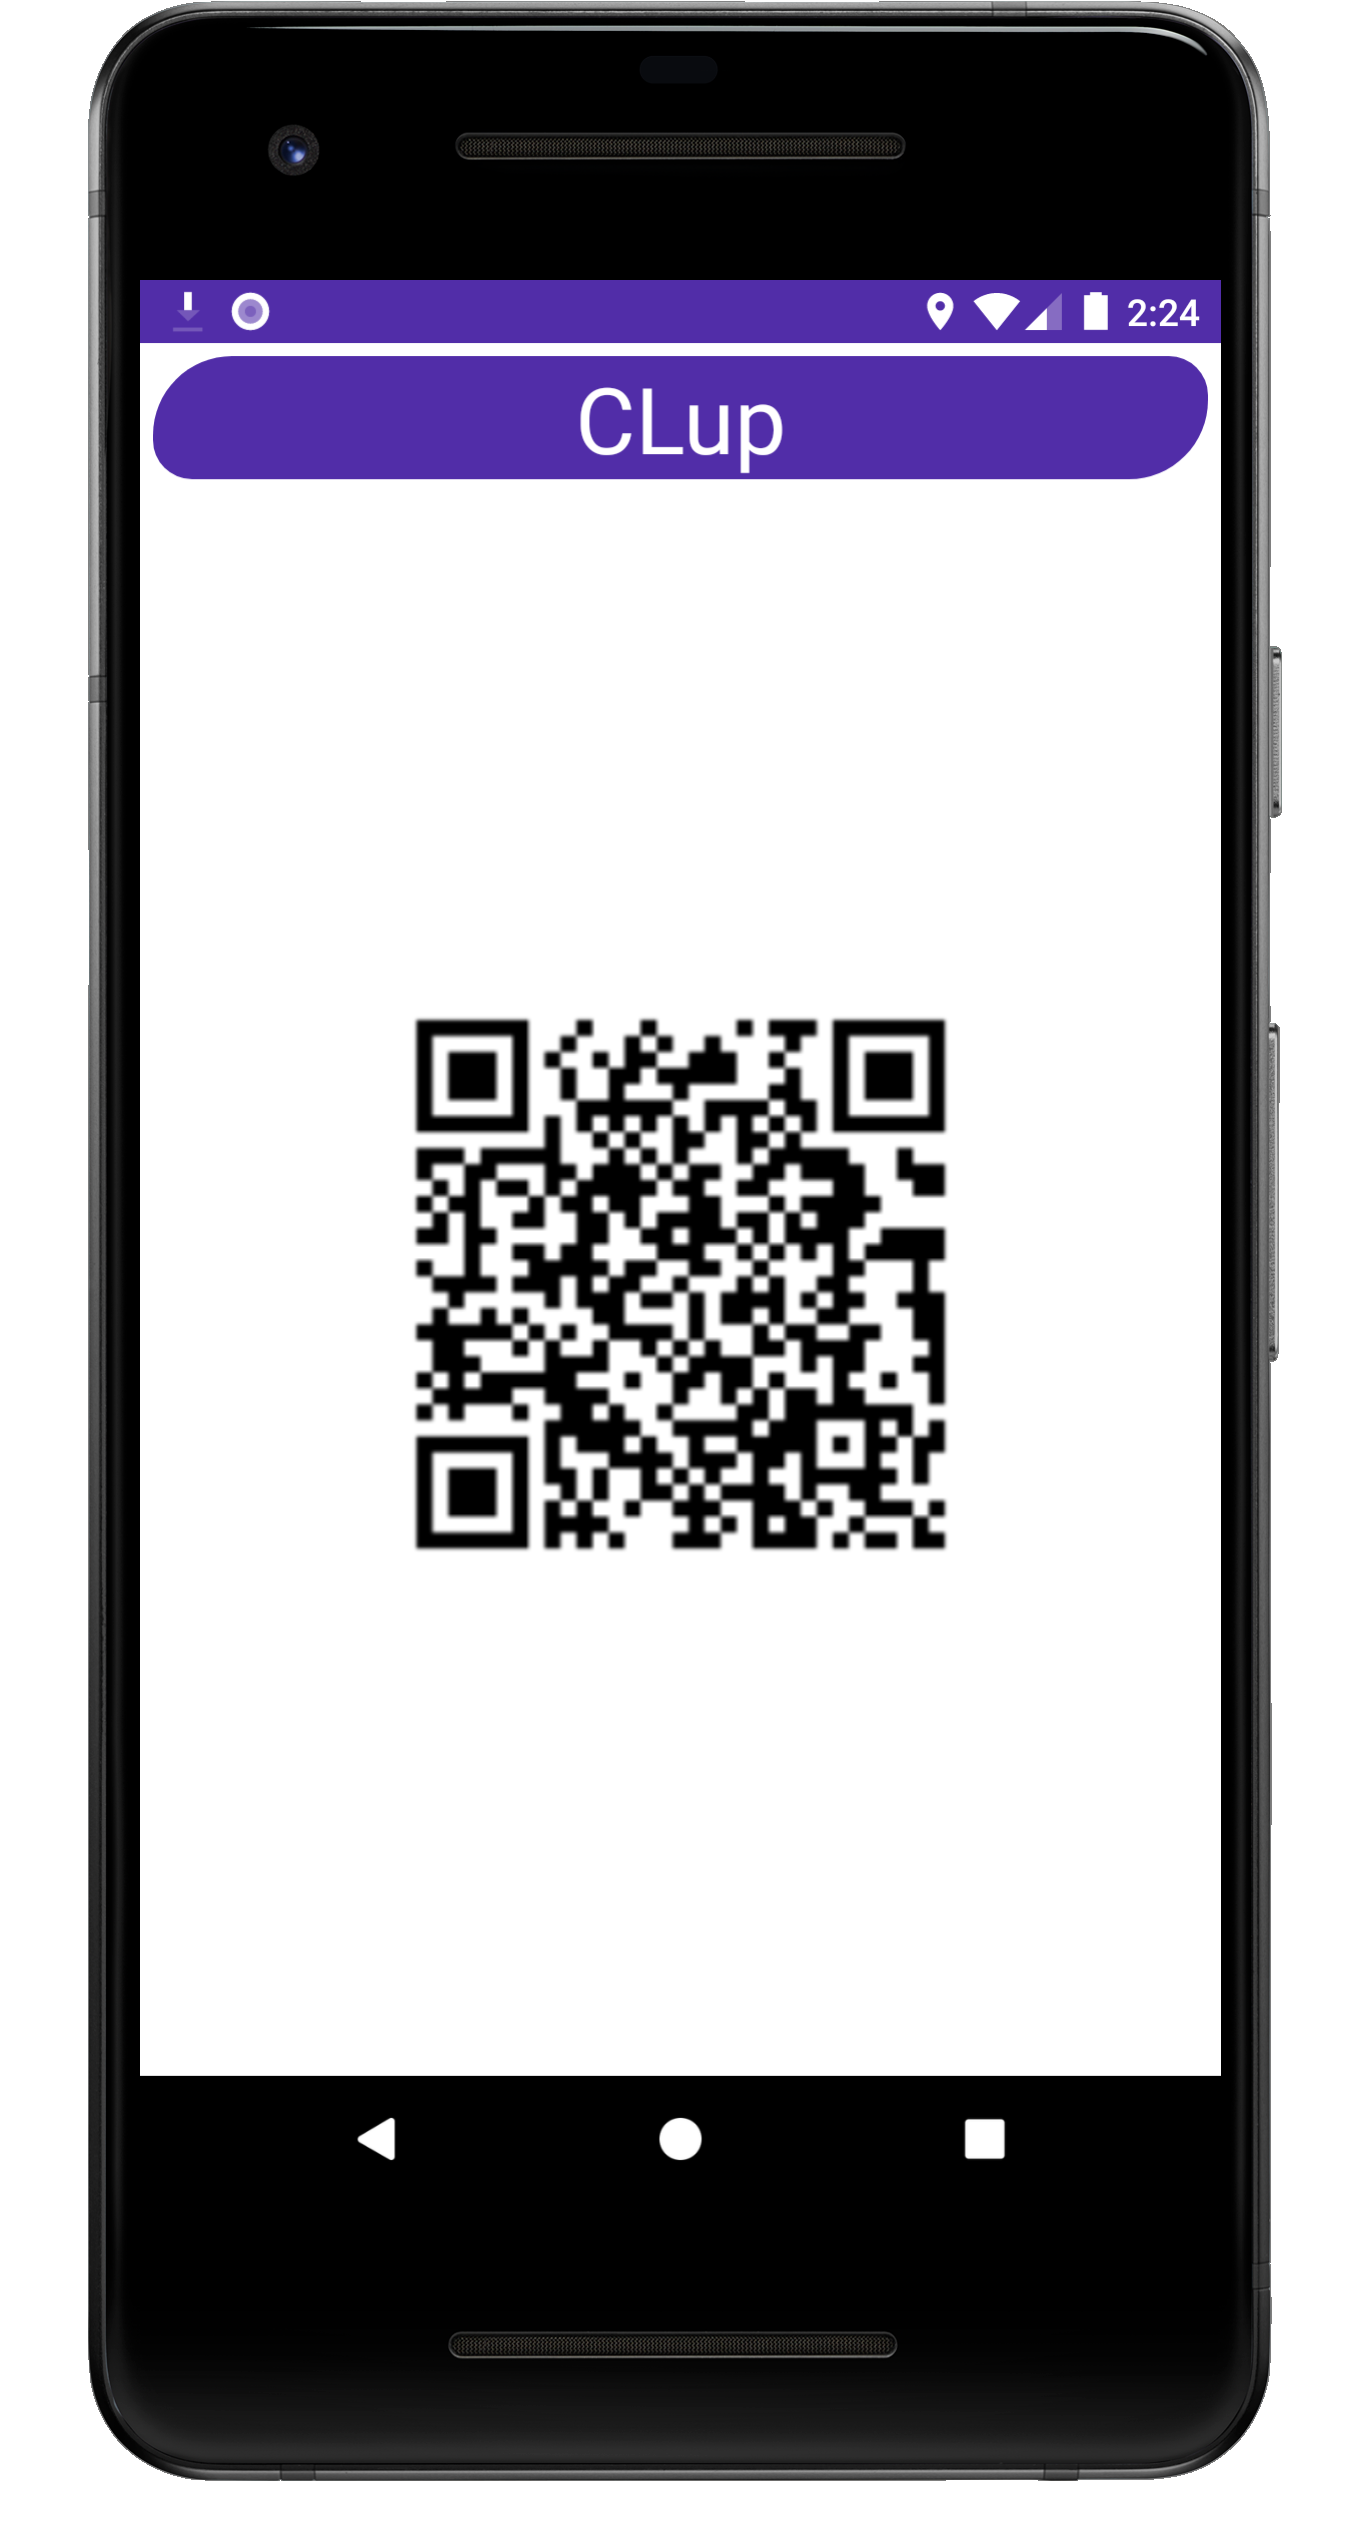
\includegraphics[width=0.4\textwidth]{images/show_qr_code.png}}
	\caption{Example of Get Status and Show QR code pages.}
\end{figure}

% TODO: add mokup for store manager

\subsection{Hardware Interfaces}

The system is distributed over three main hardware resources.

\begin{itemize}
	\item \textbf{Smartphone}: used by the customers that wants to line up or book a visit from remote. The smartphone has to have a \gls{gps} module to send the position and an Internet connection active to receive live updates by the server.
	\item \textbf{Physical spot}: is a totem composed by a tablet and a printer. The printer is a peripheral of the tablet. The tablet must have an Internet connection active.
	\item \textbf{Turnstile}: is used to control the entries. The tablet of the store manager, the QR code scanner and the display, that shows the next ticket numbers, are parts of the turnstile. More precisely, turnstile, scanner and display are peripherals of the tablet.
	We can imagine the turnstile as the metal detector in the airports, in which the guards are seated on the opposite side of the entrance.
	The store manager controls everything by the tablet and the tablet controls the peripherals under the constraints imposed by the store manager and the remote server.
	Indeed the tablet has to have an Internet connection active.
\end{itemize}

\subsection{Software interfaces}

The system, to work properly, needs external \gls{api}.

\begin{itemize}
	\item \textbf{Store \glspl{api}}: are well-liked if they there are. Additional data provided by the store, such as the history of the purchases of the customers, can be used to improve the quality of the estimations of the residence time; the sections of the store that will be visited by customers and so on.
	\item \textbf{Maps \glspl{api}}: can be used to improve the estimation of the needed time to arrive to the store by the global position of the customer.
\end{itemize}

\subsection{Communications Interfaces}

In this service we aren't not scheduling to use external communications interfaces.
Only the standard Internet protocols.

\section{Functional Requirements}

\subsection{Requirements}

Bla bla bla...

\begin{table}[H]
\centering
\begin{tabular}{| m{0.2\textwidth} | m{0.8\textwidth} |} 
	\hline
	\textbf{Goal} &
		\textbf{G1: Keep customers in safe condition w.r.t the \gls{dpcm} in force inside the store.} \\
	\hline
	\textbf{Requirements} &
		\begin{itemize}
			\item {\textbf{[R1]}}: The system has to schedule entrances to the store.
			\item {\textbf{[R2]}}: The system has to compute the maximum capacity of the store w.r.t. the social distances imposed by the \gls{dpcm} in force.
			\item {\textbf{[R3]}}: The system has to monitor the customers residence time in the store.
			\item {\textbf{[R4]}}: The system has to allow authorized customers to enter in the store.
			\item {\textbf{[R5]}}: The system has to deny unauthorized customers to enter in the store.
			\item {\textbf{[R6]}}: The system has to know when a customer enters in the store.
			\item {\textbf{[R7]}}: The system has to know when a customer has left the store.
		\end{itemize} \\
	\hline
	\shortstack[l]{\textbf{Domain} \\ \textbf{Assumptions}} & 
		\begin{itemize}
			\item {\textbf{[D1]}}: There is a \gls{dpcm} in force.
			\item {\textbf{[D2]}}: Customers follow the rules imposed by the \gls{dpcm} in force.
			\item {\textbf{[D3]}}: Customers enter in the store only if the system authorizes them.
			\item {\textbf{[D4]}}: Customers don't stay in the shop longer than necessary and they go away from the store after they have done their shopping.
			% \item {\textbf{[D]}}: If customers booked a visit to the store and they specify the category of grocery, they won't buy other things.
		\end{itemize} \\ 
	\hline
\end{tabular}
\end{table}

\begin{table}[H]
\centering
\begin{tabular}{| m{0.2\textwidth} | m{0.8\textwidth} |} 
	\hline
	\textbf{Goal} &
		\textbf{G2: Limit the physical line situation in the proximity of the store} \\
	\hline
	\textbf{Requirements} &
		\begin{itemize}
			\item {\textbf{[R8]}}: The system has to estimate the residence time, of a customer, in the store.
			\item {\textbf{[R9]}}: The system has to infer the residence time of the customers based on past purchases.
			\item {\textbf{[R10]}}: The system has to estimate the time needed to arrive, to the store, from the position of the customer.
			\item {\textbf{[R11]}}: The system has to track the global position of the customers.
			\item {\textbf{[R12]}}: The system has to release QR codes to the customers.
			\item {\textbf{[R13]}}: The system has to limit the number of releasable QR codes if imposed by the store manager.
			\item {\textbf{[R14]}}: The system has to allow the store manager to monitor the status of the queue.
			\item {\textbf{[R15]}}: The system has to notify customers about the remaining time to be authorized to enter in the store.
			\item {\textbf{[R16]}}: The system has to communicate which is the next served QR code number.
		\end{itemize} \\ 
	\hline
	\shortstack[l]{\textbf{Domain} \\ \textbf{Assumptions}} & 
		\begin{itemize}
			\item {\textbf{[D5]}}: Customers line up physically only if they have a valid (non expired) QR code.
			\item {\textbf{[D4]}}: Customers don't stay in the shop longer than necessary and they go away from the store after they have done their shopping.
			\item {\textbf{[D6]}}: Outside the store there is space to queue.
		\end{itemize} \\ 
	\hline
\end{tabular}
\end{table}

\begin{table}[H]
\centering
\begin{tabular}{| m{0.2\textwidth} | m{0.8\textwidth} |} 
	\hline
	\textbf{Goal} &
		\textbf{G3: Allow customers to line up from a remote device.} \\
		% requirements per l'app e il servizio di prenotazione (quality standard)
	\hline
	\textbf{Requirements} &
		\begin{itemize}
			\item {\textbf{[R17]}}: The system has to allow customers to register to the application.
			\item {\textbf{[R18]}}: The system has to allow customers to login to the application.
			\item {\textbf{[R19]}}: The system has to allow customers to get a QR code from the application.
			\item {\textbf{[R20]}}: The system has to release QR codes to the customers through the application.
			\item {\textbf{[R21]}}: The system has to alert customers if the queue is full.
			\item {\textbf{[R22]}}: The system has to encode the lining up number in the QR code.
			\item {\textbf{[R23]}}: The system has to allow customers to watch the QR code from the application.
			\item {\textbf{[R24]}}: The system has to allow customers to watch the lining up number encoded in the QR code.
			\item {\textbf{[R25]}}: The system has to allow customers to watch the remaining time to be authorized to enter in the store.
			\item {\textbf{[R26]}}: The system has to update the remaining time showed to the customers.
			\item {\textbf{[R27]}}: The system has to allow customers to delete a lining up operation.
			\item {\textbf{[R28]}}: The system has to notify customers about the validation status of the QR code.
			\item {\textbf{[R29]}}: The system has to check if customers have Internet connection active.
			\item {\textbf{[R30]}}: The system has to check if customers have allowed the permissions requested by the application.
		\end{itemize} \\ 
	\hline
	\shortstack[l]{\textbf{Domain} \\ \textbf{Assumptions}} & 
		\begin{itemize}
			\item {\textbf{[D7]}}: Customers have a smartphone.
			\item {\textbf{[D8]}}: Customers have installed the \gls{clup} application.
			\item {\textbf{[D9]}}: Customers allow the permissions requested by the application.
			\item {\textbf{[D10]}}: Customers keep Internet connection active.
		\end{itemize} \\ 
	\hline
\end{tabular}
\end{table}

\begin{table}[H]
\centering
\begin{tabular}{| m{0.2\textwidth} | m{0.8\textwidth} |} 
	\hline
	\textbf{Goal} &
		\textbf{G4: Allow store manager to monitor entrances.} \\
	\hline
	\textbf{Requirements} &
		\begin{itemize}
			\item {\textbf{[R31]}}: The system has to register store managers in the application.
			\item {\textbf{[R32]}}: The system has to allow store managers to login to the application.
			\item {\textbf{[R33]}}: The system has to allow store managers to monitor the status of the queue.
			\item {\textbf{[R34]}}: The system has to allow store managers to limit the number of QR codes released.
			\item {\textbf{[R35]}}: The system has to allow store managers to monitor the number of customers inside the store.
			\item {\textbf{[R36]}}: The system has to scan the QR codes of the customers.
			\item {\textbf{[R37]}}: The system has to allow store managers to modify the timing parameters of the scheduler.
			\item {\textbf{[R38]}}: The system has to check if store managers have Internet connection active.
			\item {\textbf{[R39]}}: The system has to check if store managers have allowed the permissions requested by the application.
		\end{itemize} \\ 
	\hline
	\shortstack[l]{\textbf{Domain} \\ \textbf{Assumptions}} & 
		\begin{itemize}
			\item {\textbf{[D11]}}: There is a store manager present in the store.
			\item {\textbf{[D12]}}: Store managers allow the permissions requested by the application.
			\item {\textbf{[D13]}}: Store managers keep Internet connection active.
		\end{itemize} \\ 
	\hline
\end{tabular}
\end{table}

\begin{table}[H]
\centering
\begin{tabular}{| m{0.2\textwidth} | m{0.8\textwidth} |} 
	\hline
	\textbf{Goal} &
		\textbf{G5: Allow customers to line up from a physical spot.} \\
	\hline
	\textbf{Requirements} &
		\begin{itemize}
			\item {\textbf{[R40]}}: The system has to allow unregistered customers to line up.
			\item {\textbf{[R41]}}: The system has to allow customers to get a QR code from a physical spot.
			\item {\textbf{[R42]}}: The system has to release QR codes to the customers through the physical spot.
			\item {\textbf{[R43]}}: The system has to encode the lining up number in the QR code.
			\item {\textbf{[R44]}}: The system has to print QR codes on a paper tickets.
			\item {\textbf{[R45]}}: The system has to alert customers if the queue is full.
			\item {\textbf{[R46]}}: The system has to alert when the paper and toner of the physical spot is going to finish.
		\end{itemize} \\ 
	\hline
	\shortstack[l]{\textbf{Domain} \\ \textbf{Assumptions}} & 
		\begin{itemize}
			\item {\textbf{[D14]}}: Physical spots are powered on every working day.
			\item {\textbf{[D15]}}: Physical spots are refilled when asked by the system. 
		\end{itemize} \\ 
	\hline
\end{tabular}
\end{table}

\begin{table}[H]
\centering
\begin{tabular}{| m{0.2\textwidth} | m{0.8\textwidth} |} 
	\hline
	\textbf{Goal} &
		\textbf{G6: Allow customers to book a visit from a remote device.} \\
		% requirements che implicano l'implementazione di una schermata nell'app per la prenotazione
	\hline
	\textbf{Requirements} &
		\begin{itemize}
			\item {\textbf{[R17]}}: The system has to allow customers to register to the application.
			\item {\textbf{[R18]}}: The system has to allow customers to login to the application.
			\item {\textbf{[R19]}}: The system has to allow customers to get a QR code from the application.
			\item {\textbf{[R47]}}: The system has to allow customers to specify the date and time for a visit to the store.
			\item {\textbf{[R48]}}: The system has to allow customers to specify the category of grocery they want to buy.
			\item {\textbf{[R20]}}: The system has to release QR codes to the customers through the application.
			\item {\textbf{[R21]}}: The system has to alert customers if the queue is full.
			\item {\textbf{[R49]}}: The system has to encode the book-a-visit number in the QR code.
			\item {\textbf{[R23]}}: The system has to allow customers to watch the QR code from the application.
			\item {\textbf{[R50]}}: The system has to allow customers to watch the book-a-visit number encoded in the QR code.
			\item {\textbf{[R25]}}: The system has to allow customers to watch the remaining time to be authorized to enter in the store.
			\item {\textbf{[R51]}}: The system has to allow customers to delete a book-a-visit operation.
			\item {\textbf{[R28]}}: The system has to notify customers about the validation status of the QR code.
			\item {\textbf{[R29]}}: The system has to check if customers have Internet connection active.
			\item {\textbf{[R30]}}: The system has to check if customers have allowed the permissions requested by the application.
		\end{itemize} \\ 
	\hline
	\shortstack[l]{\textbf{Domain} \\ \textbf{Assumptions}} & 
		\begin{itemize}
			\item {\textbf{[D7]}}: Customers have a smartphone.
			\item {\textbf{[D8]}}: Customers have installed the \gls{clup} application.
			\item {\textbf{[D9]}}: Customers allow the permissions requested by the application.
			\item {\textbf{[D10]}}: Customers keep Internet connection active.
		\end{itemize} \\ 
	\hline
\end{tabular}
\end{table}


\subsection{Definition of Use Case Diagrams}

Bla bla bla...

\begin{figure}[H]
	\centering
	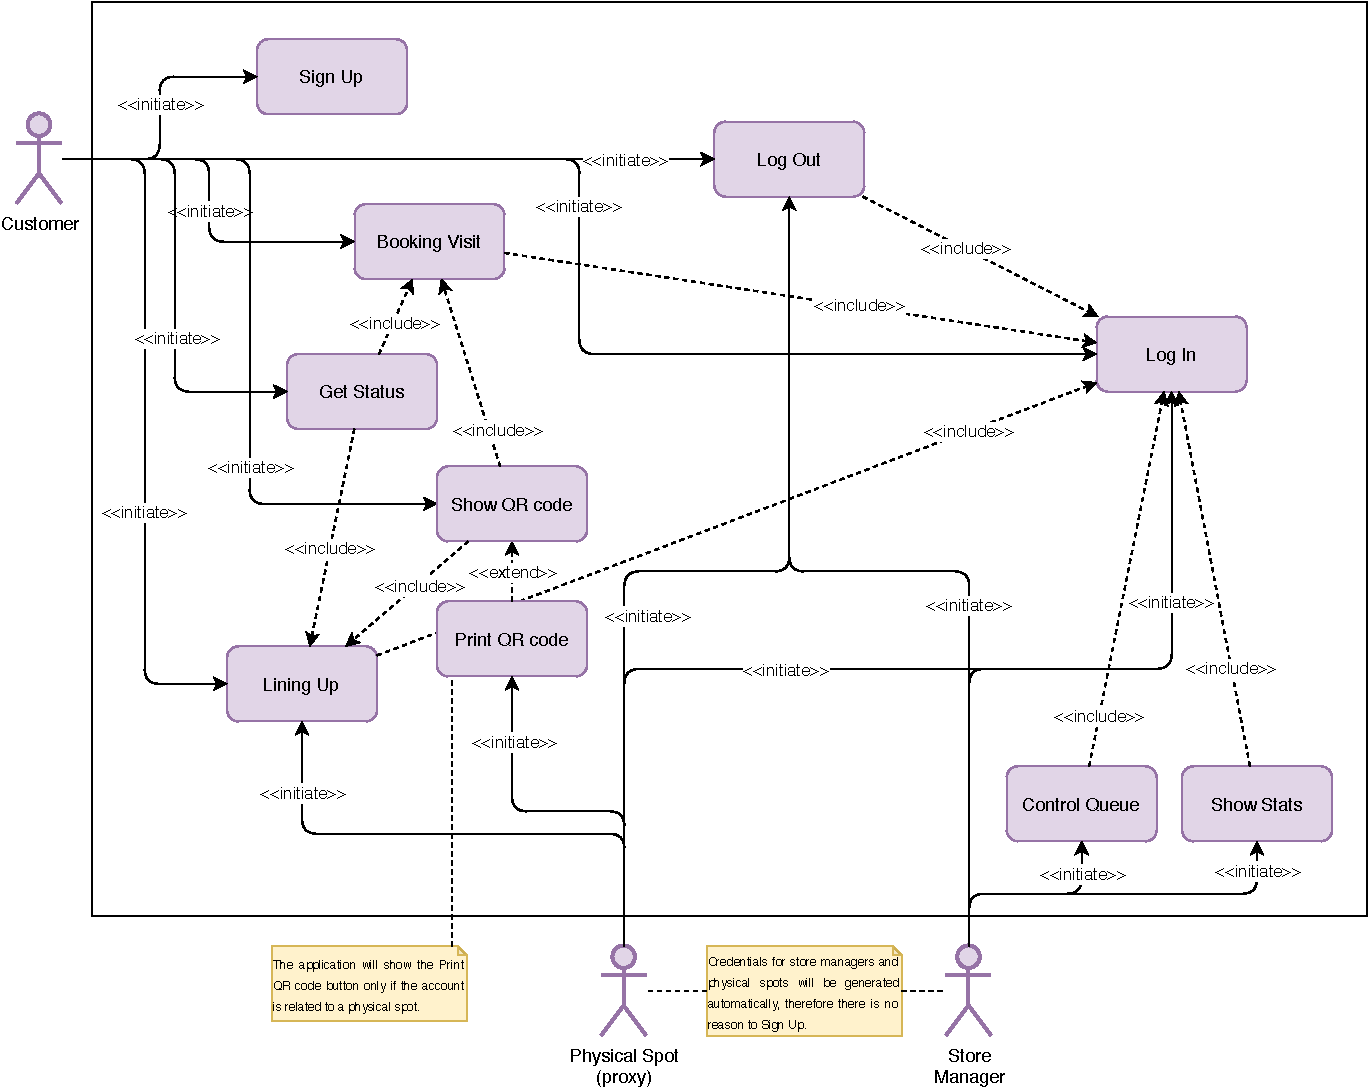
\includegraphics[width=1.0\textwidth]{images/use_cases_diagram.pdf}
	\caption{Use cases diagram.}
\end{figure}

\begin{table}[H]
\centering
\begin{tabular}{| m{0.3\textwidth} | m{0.7\textwidth} |} 
	\hline
	\textbf{Name} & Sign Up \\ 
	\hline
	\textbf{Actor} & Customer \\ 
	\hline
	\textbf{Entry Conditions} & Customer is on the Sign Up page. \\ 
	\hline
	\textbf{Event Flows} &
	\begin{itemize}
		\item Customer inserts the requested information in the form.
		\item Customer clicks on the Sign Up button.
	\end{itemize} \\ 
	\hline
	\textbf{Exit Conditions} & Sign Up completed successfully and customer is logged in, then the application shows the Home page. \\ 
	\hline
	\textbf{Exceptions} &
	\begin{itemize}
		\item Customer's username already in use.
		\item Empty form field.
		\item Policy agreement rejected.
		\item Lost Internet connection.
	\end{itemize} \\ 
	\hline
\end{tabular}
\caption{Use case: \textbf{Sign Up}.}
\label{tableSignUp}
\end{table}

\begin{table}[H]
\centering
\begin{tabular}{| m{0.3\textwidth} | m{0.7\textwidth} |} 
	\hline
	\textbf{Name} & Log In \\ 
	\hline
	\textbf{Actor} & Customer - Physical Spot - Store Manager \\ 
	\hline
	\textbf{Entry Conditions} & Actor is on the Log In page. \\ 
	\hline
	\textbf{Event Flows} &
	\begin{itemize}
	\item Actor inserts the requested information in the form.
	\item Actor clicks on the Log In button.
	\end{itemize} \\ 
	\hline
	\textbf{Exit Conditions} & Log In completed successfully and actor is redirected to the Home page. \\ 
	\hline
	\textbf{Exceptions} &
	\begin{itemize}
	\item Actor's username or password incorrect.
	\item Empty form field.
	\item Lost Internet connection.
	\end{itemize} \\ 
	\hline
\end{tabular}
\caption{Use case: \textbf{Log In}.}
\label{tableLogIn}
\end{table}

\begin{table}[H]
\centering
\begin{tabular}{| m{0.3\textwidth} | m{0.7\textwidth} |} 
	\hline
	\textbf{Name} & Log Out \\ 
	\hline
	\textbf{Actor} & Customer - Physical Spot - Store Manager \\ 
	\hline
	\textbf{Entry Conditions} & Actor is on the Log Out page. \\ 
	\hline
	\textbf{Event Flows} &
	\begin{itemize}
	\item Actor clicks on the Log Out button.
	\end{itemize} \\ 
	\hline
	\textbf{Exit Conditions} & Log Out completed successfully and actor is redirected to the Log In page. \\ 
	\hline
	\textbf{Exceptions} &
	\begin{itemize}
	\item Actor already logged out.
	\item Lost Internet connection.
	\end{itemize} \\ 
	\hline
\end{tabular}
\caption{Use case: \textbf{Log Out}.}
\label{tableLogOut}
\end{table}

\begin{table}[H]
\centering
\begin{tabular}{| m{0.3\textwidth} | m{0.7\textwidth} |} 
	\hline
	\textbf{Name} & Lining Up \\ 
	\hline
	\textbf{Actor} & Customer - Physical Spot \\ 
	\hline
	\textbf{Entry Conditions} & Actor is on the Home page. \\ 
	\hline
	\textbf{Event Flows} &
	\begin{itemize}
	\item Actor clicks on the Lining Up button.
	\item Actor inserts the requested data in the form.
	\item Actor clicks on the confirmation button.
	\end{itemize} \\ 
	\hline
	\textbf{Exit Conditions} & Lining Up completed successfully, the application returns the Status page. \\ 
	\hline
	\textbf{Exceptions} &
	\begin{itemize}
	\item Previous Lining Up action was not expired (only in case of remote customer).
	\item Previous Booking Visit action was not expired (only in case of remote customer).
	\item Actor wasn't logged.
	\item Lost Internet connection.
	\end{itemize} \\ 
	\hline
\end{tabular}
\caption{Use case: \textbf{Lining Up}.}
\label{tableLiningUp}
\end{table}

\begin{table}[H]
\centering
\begin{tabular}{| m{0.3\textwidth} | m{0.7\textwidth} |} 
	\hline
	\textbf{Name} & Booking Visit \\ 
	\hline
	\textbf{Actor} & Customer \\ 
	\hline
	\textbf{Entry Conditions} & Customer is on the Home page. \\ 
	\hline
	\textbf{Event Flows} &
	\begin{itemize}
	\item Customer clicks on the Booking Visit button.
	\item Customer fills the form with the requested data.
	\item Customer clicks on the Submit button.
	\end{itemize} \\ 
	\hline
	\textbf{Exit Conditions} & Booking Visit completed successfully and the application returns, to the customer, the Status page. \\ 
	\hline
	\textbf{Exceptions} &
	\begin{itemize}
	\item Previous Lining Up action was not expired.
	\item Previous Booking Visit action was not expired.
	\item Customer wasn't logged.
	\item Lost Internet connection.
	\end{itemize} \\ 
	\hline
\end{tabular}
\caption{Customer - use case: \textbf{Booking Visit}.}
\label{tableBookingVisit}
\end{table}

\begin{table}[H]
\centering
\begin{tabular}{| m{0.3\textwidth} | m{0.7\textwidth} |} 
	\hline
	\textbf{Name} & Show QR code - Print QR code \\ 
	\hline
	\textbf{Actor} & Customer - Physical Spot \\ 
	\hline
	\textbf{Entry Conditions} & Actor is on the Home page. \\ 
	\hline
	\textbf{Event Flows} &
	\begin{itemize}
	\item Actor clicks on the Show QR (Print QR) code button.
	\end{itemize} \\ 
	\hline
	\textbf{Exit Conditions} & The application shows (print) the QR code. \\ 
	\hline
	\textbf{Exceptions} &
	\begin{itemize}
	\item QR code wasn't saved on the application correctly (only in case of remote customer).
	\item No Lining Up, or Booking Visit, action previously performed (only in case of remote customer).
	\item Actor wasn't logged.
	\item Spot finished the paper.
	\item Spot finished the ink.
	\end{itemize} \\ 
	\hline
\end{tabular}
\caption{Use case: \textbf{Show QR code - Print QR code}.}
\label{tableShowQR}
\end{table}

\begin{table}[H]
\centering
\begin{tabular}{| m{0.3\textwidth} | m{0.7\textwidth} |} 
	\hline
	\textbf{Name} & Get Status \\ 
	\hline
	\textbf{Actor} & Customer \\ 
	\hline
	\textbf{Entry Conditions} & Customer is on the Home page. \\ 
	\hline
	\textbf{Event Flows} &
	\begin{itemize}
	\item Customer clicks on the Get Status button.
	\end{itemize} \\ 
	\hline
	\textbf{Exit Conditions} & The application returns the Get Status page showing information about the last Lining Up, or Booking Visit, operation. \\ 
	\hline
	\textbf{Exceptions} &
	\begin{itemize}
	\item No operation previously performed, therefore there is no data to show.
	\item Customer wasn't logged.
	\item Lost Internet connection.
	\end{itemize} \\ 
	\hline
\end{tabular}
\caption{Customer - use case: \textbf{Get Status}.}
\label{tableGetStatus}
\end{table}

\begin{table}[H]
\centering
\begin{tabular}{| m{0.3\textwidth} | m{0.7\textwidth} |} 
	\hline
	\textbf{Name} & Control Queue \\ 
	\hline
	\textbf{Actor} & Store Manager \\ 
	\hline
	\textbf{Entry Conditions} & Store Manager is on the Home page. \\ 
	\hline
	\textbf{Event Flows} &
	\begin{itemize}
	\item Store Manager clicks on the Control Queue button.
	\end{itemize} \\ 
	\hline
	\textbf{Exit Conditions} & The application returns the Control Queue page showing options to manage the queue. \\ 
	\hline
	\textbf{Exceptions} &
	\begin{itemize}
	\item Store Manager wasn't logged.
	\item Lost Internet connection.
	\end{itemize} \\ 
	\hline
\end{tabular}
\caption{Store Manager - use case: \textbf{Control Queue}.}
\label{tableGetStatus}
\end{table}

\begin{table}[H]
\centering
\begin{tabular}{| m{0.3\textwidth} | m{0.7\textwidth} |} 
	\hline
	\textbf{Name} & Show Stats \\ 
	\hline
	\textbf{Actor} & Store Manager \\ 
	\hline
	\textbf{Entry Conditions} & Store Manager is on the Home page. \\ 
	\hline
	\textbf{Event Flows} &
	\begin{itemize}
	\item Store Manager clicks on the Show Stats button.
	\end{itemize} \\ 
	\hline
	\textbf{Exit Conditions} & The application returns the Show Stats page showing information about the number of customers inside the store, the length of the queue and other information about the waiting time in queue. \\ 
	\hline
	\textbf{Exceptions} &
	\begin{itemize}
	\item Store Manager wasn't logged.
	\item Lost Internet connection.
	\end{itemize} \\ 
	\hline
\end{tabular}
\caption{Store Manager - use case: \textbf{Show Stats}.}
\label{tableGetStatus}
\end{table}


\subsection{Use Cases and Sequence/Activity Diagrams}

\begin{figure}[H]
	\centering
	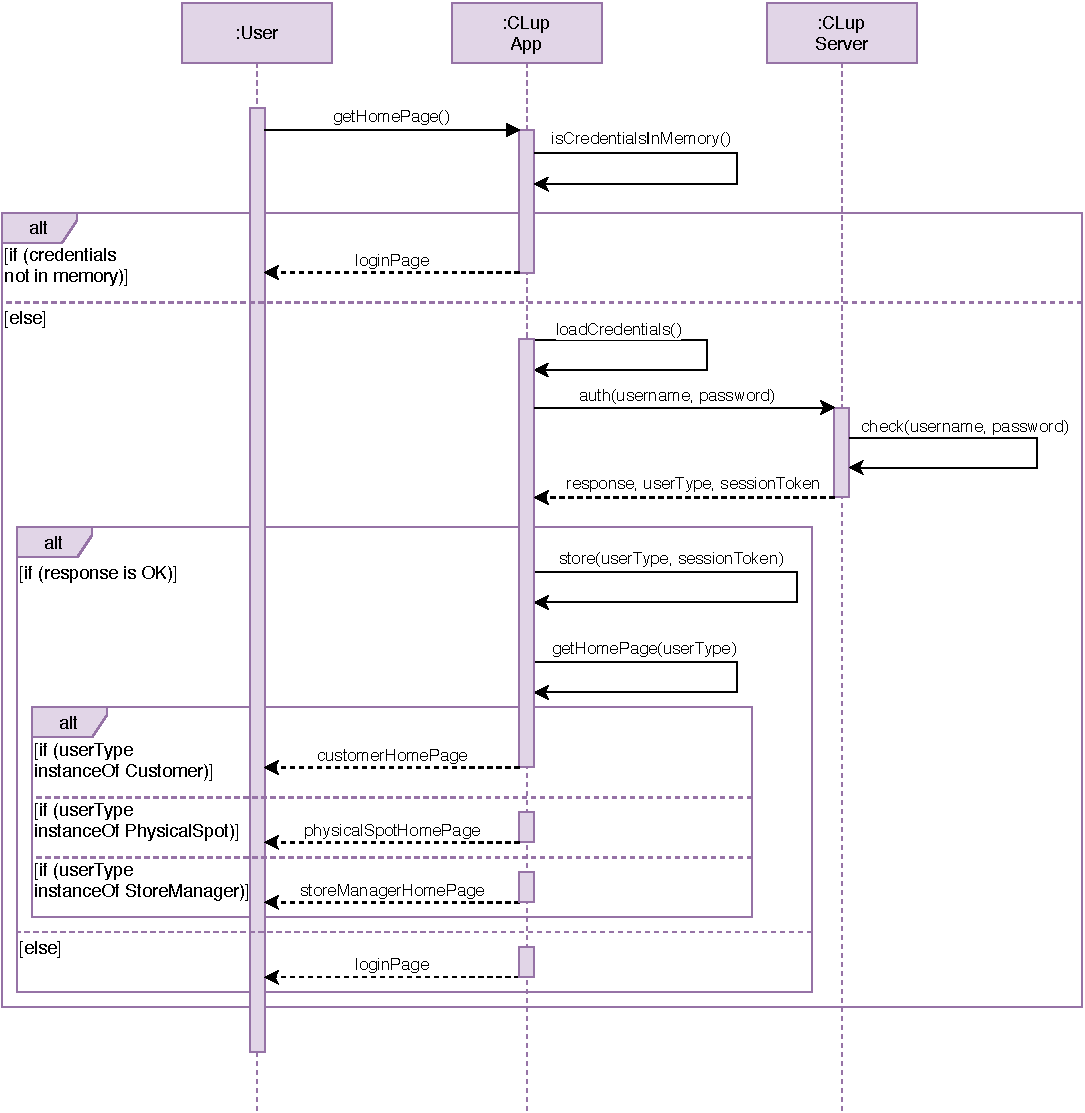
\includegraphics[width=1.0\textwidth]{images/getHomePage_sequence_diagram.pdf}
	\caption{Home page sequence diagram.}
\end{figure}

\begin{figure}[H]
	\centering
	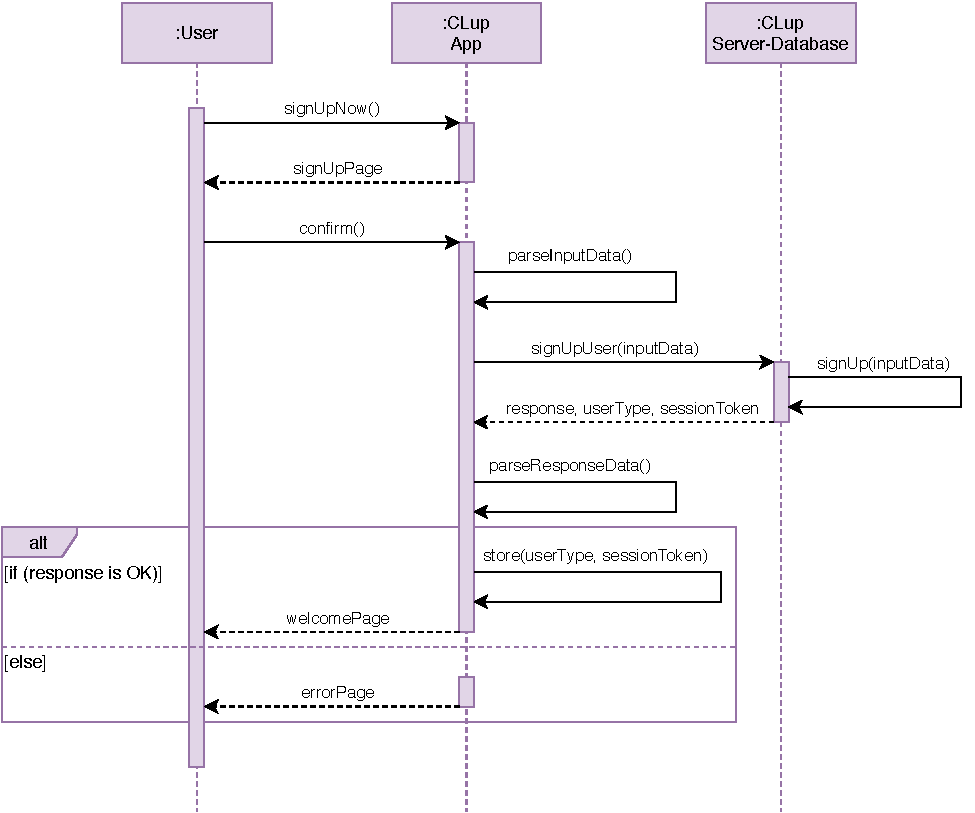
\includegraphics[width=1.0\textwidth]{images/signUp_sequence_diagram.pdf}
	\caption{Sign Up sequence diagram.}
\end{figure}

\begin{figure}[H]
	\centering
	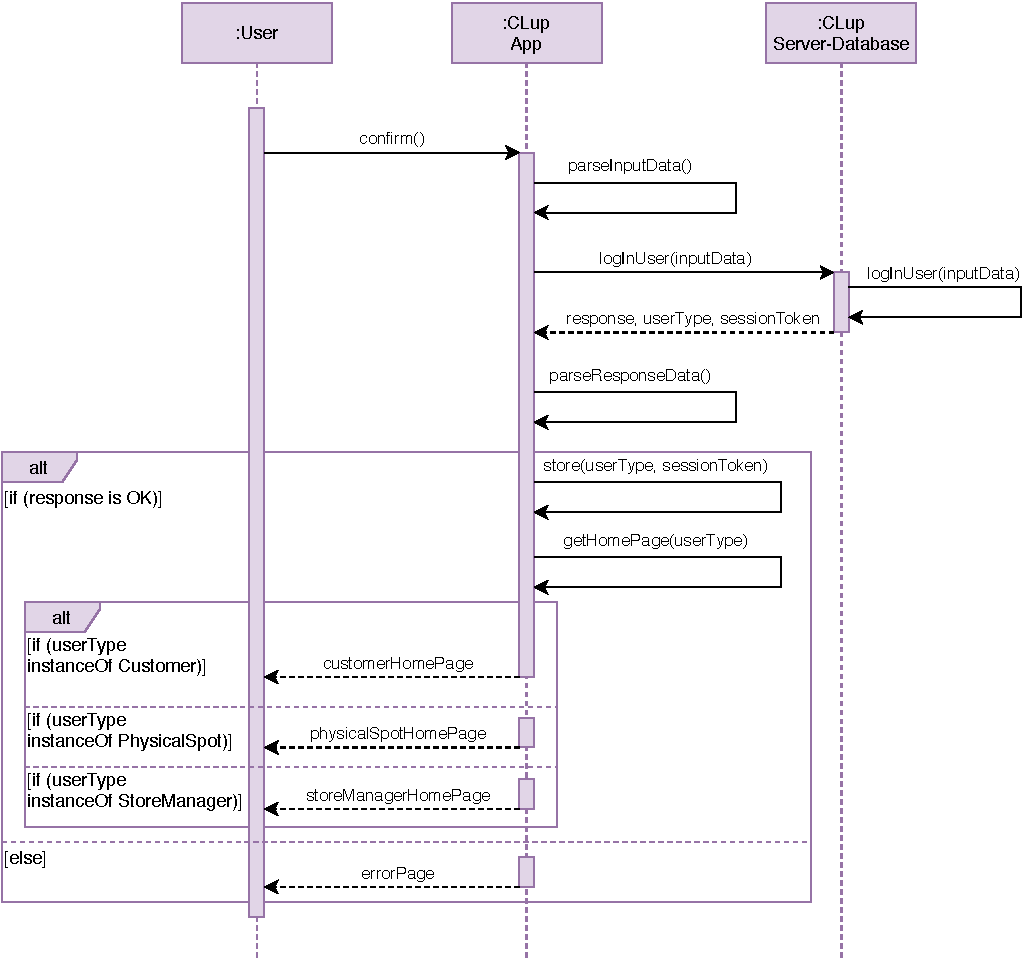
\includegraphics[width=1.0\textwidth]{images/logIn_sequence_diagram.pdf}
	\caption{Log In sequence diagram.}
\end{figure}

\begin{figure}[H]
	\centering
	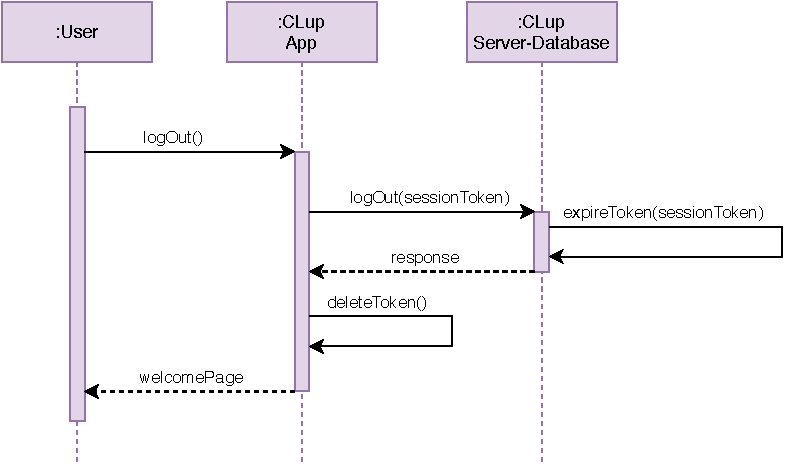
\includegraphics[width=1.0\textwidth]{images/logOut_sequence_diagram.pdf}
	\caption{Log Out sequence diagram.}
\end{figure}

\begin{figure}[H]
	\centering
	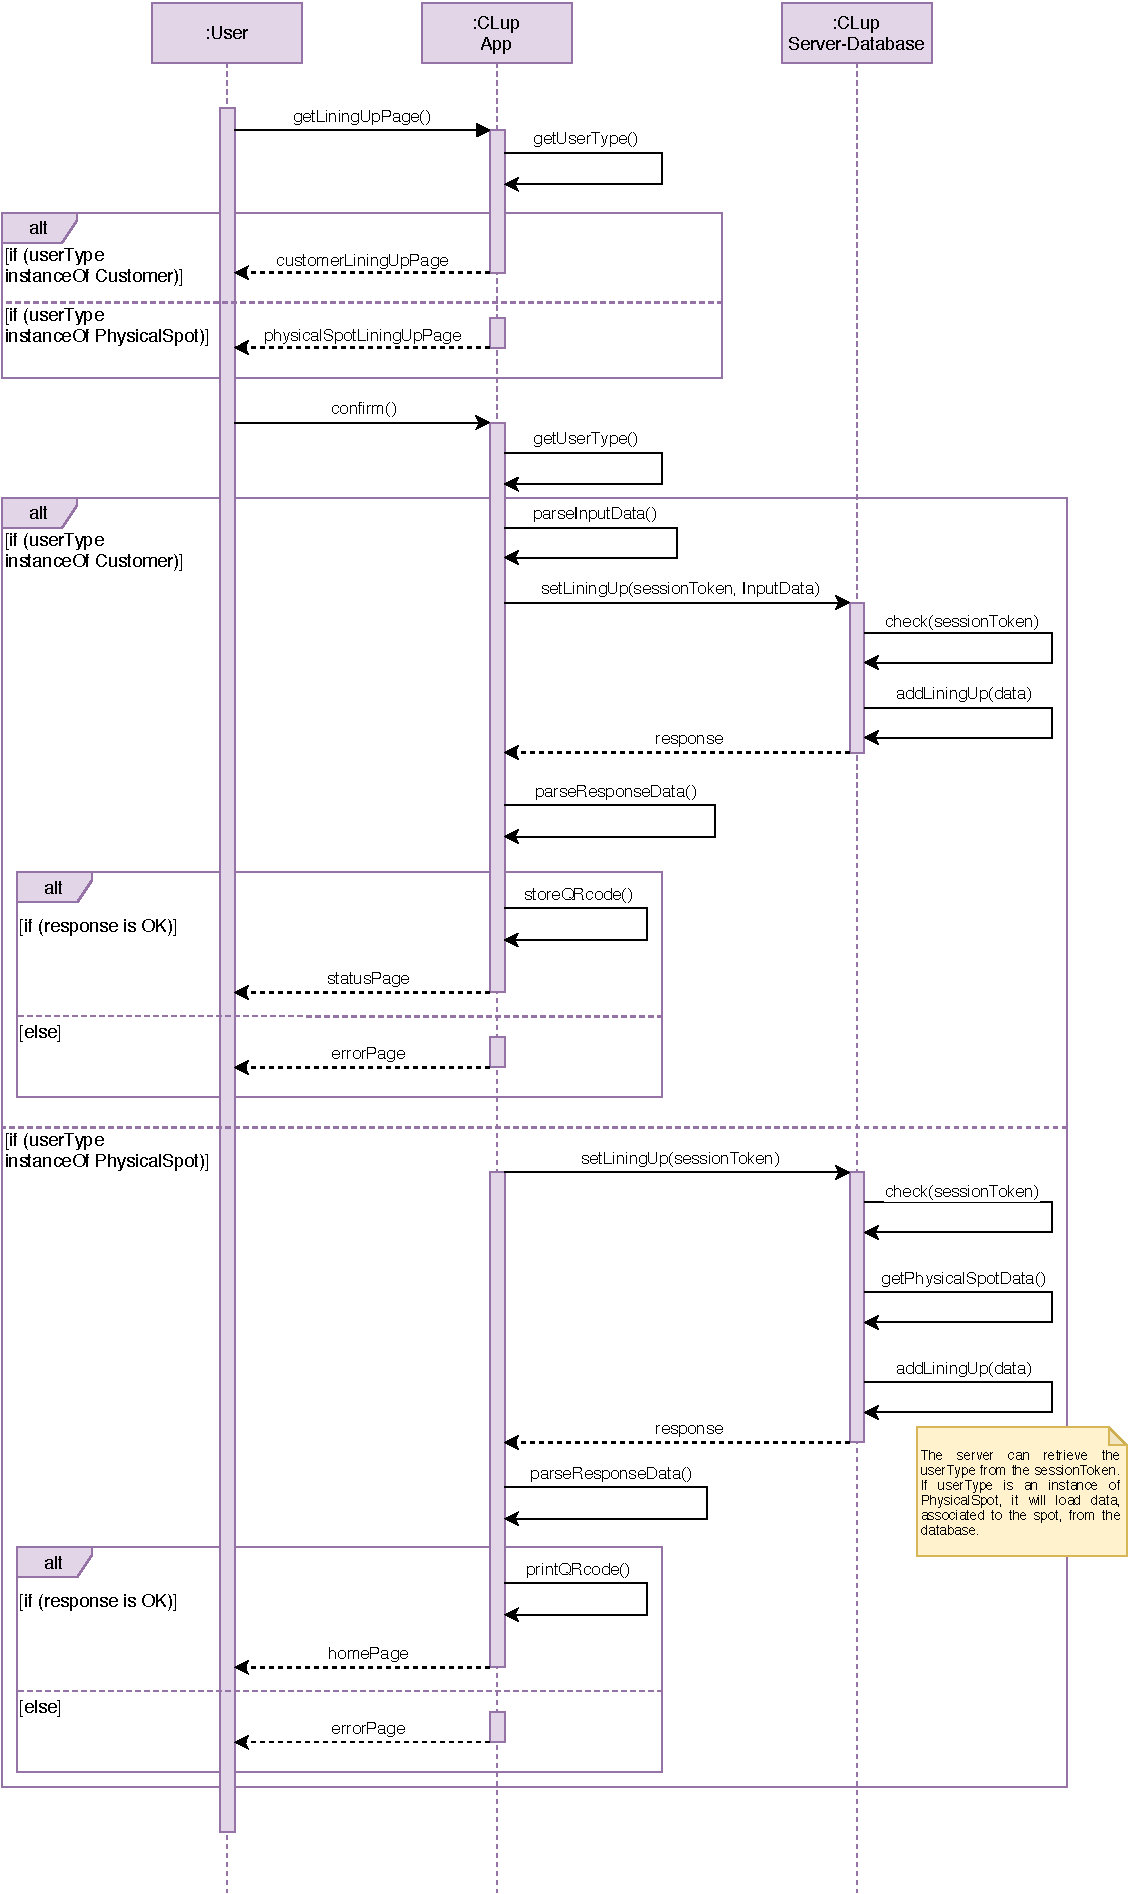
\includegraphics[width=1.0\textwidth]{images/liningUp_sequence_diagram.pdf}
	\caption{Lining Up sequence diagram.}
	\label{figure:liningUpSequenceDiagram}
\end{figure}

\begin{figure}[H]
	\centering
	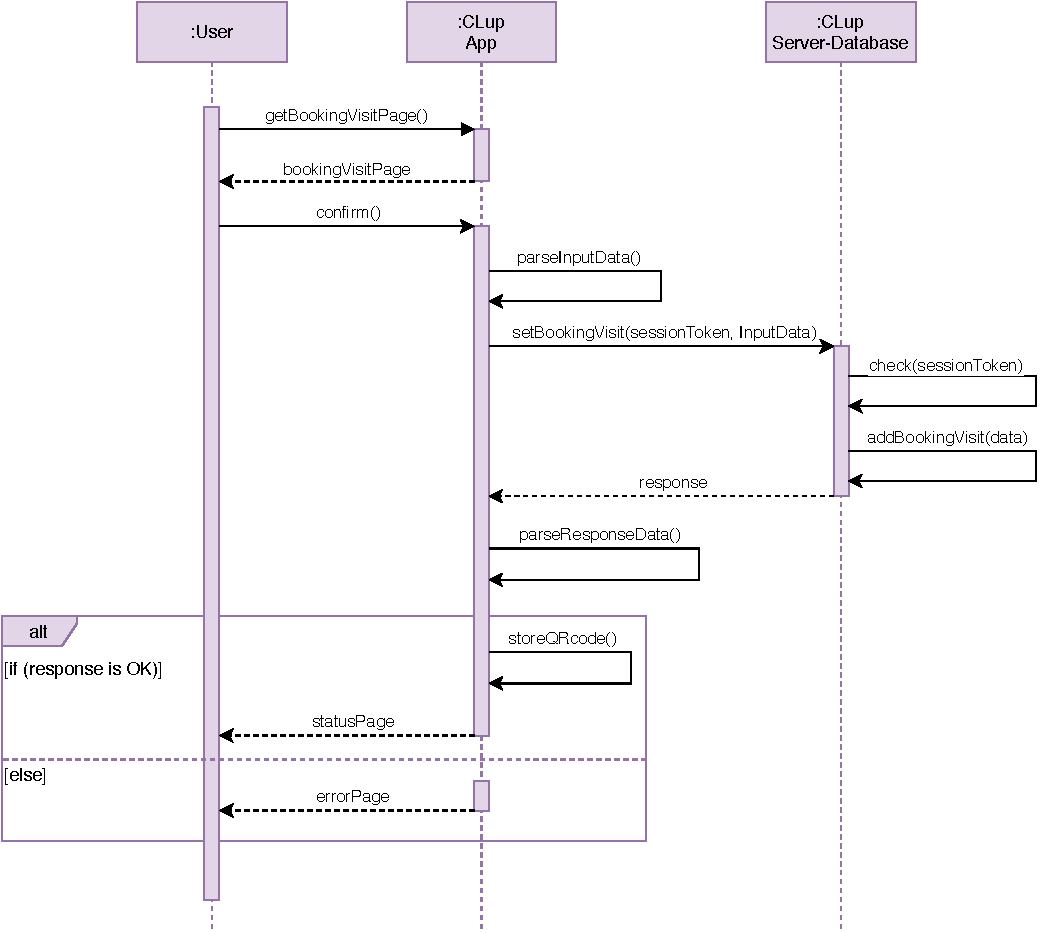
\includegraphics[width=1.0\textwidth]{images/bookingVisit_sequence_diagram.pdf}
	\caption{Booking a Visit sequence diagram.}
\end{figure}

\begin{figure}[H]
	\centering
	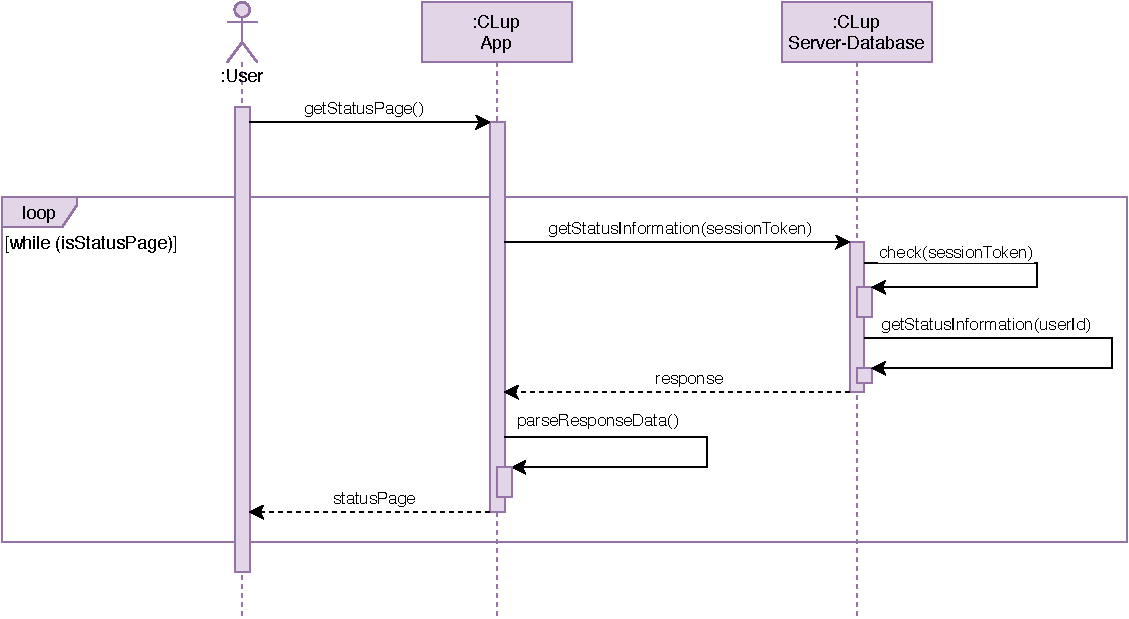
\includegraphics[width=1.0\textwidth]{images/getStatusPage_sequence_diagram.pdf}
	\caption{Get Status sequence diagram.}
\end{figure}

\begin{figure}[H]
	\centering
	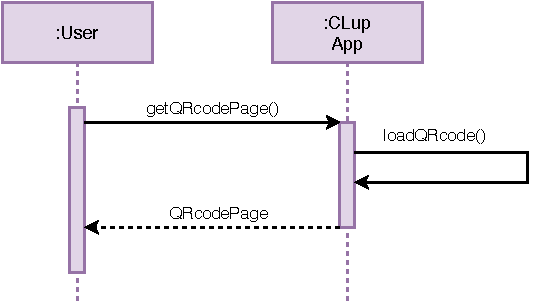
\includegraphics[width=1.0\textwidth]{images/getQRcodePage_sequence_diagram.pdf}
	\caption{QR code page sequence diagram.}
\end{figure}

\begin{figure}[H]
	\centering
	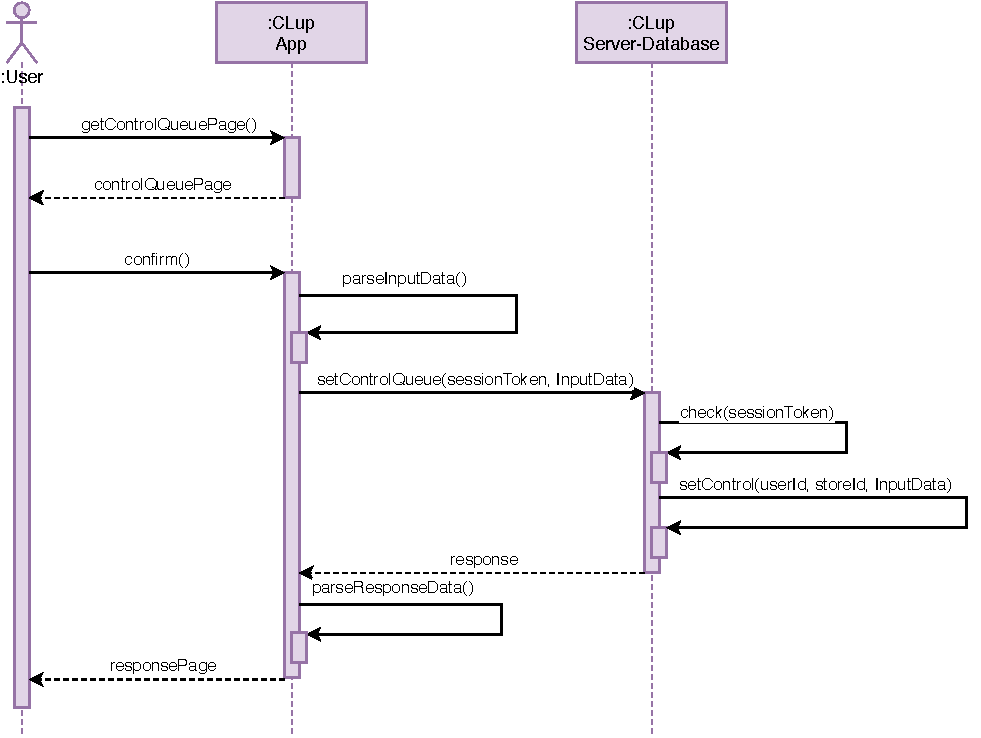
\includegraphics[width=1.0\textwidth]{images/getControlQueuePage_sequence_diagram.pdf}
	\caption{Control Queue sequence diagram.}
\end{figure}

\begin{figure}[H]
	\centering
	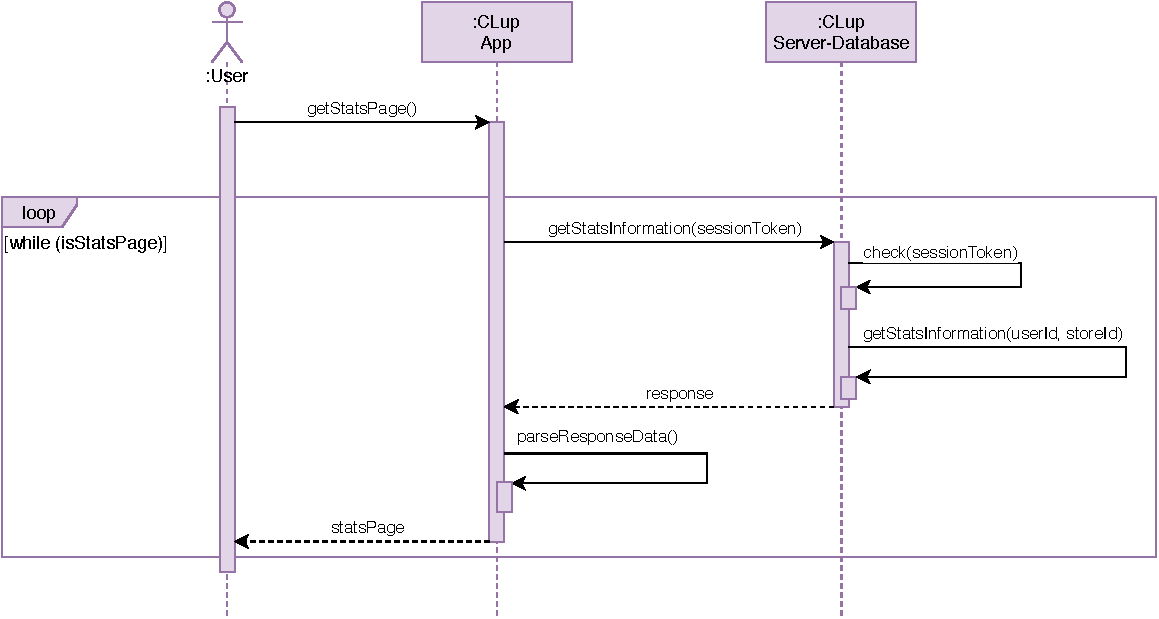
\includegraphics[width=1.0\textwidth]{images/getShowStatsPage_sequence_diagram.pdf}
	\caption{Show Stats sequence diagram.}
\end{figure}

\begin{figure}[H]
	\centering
	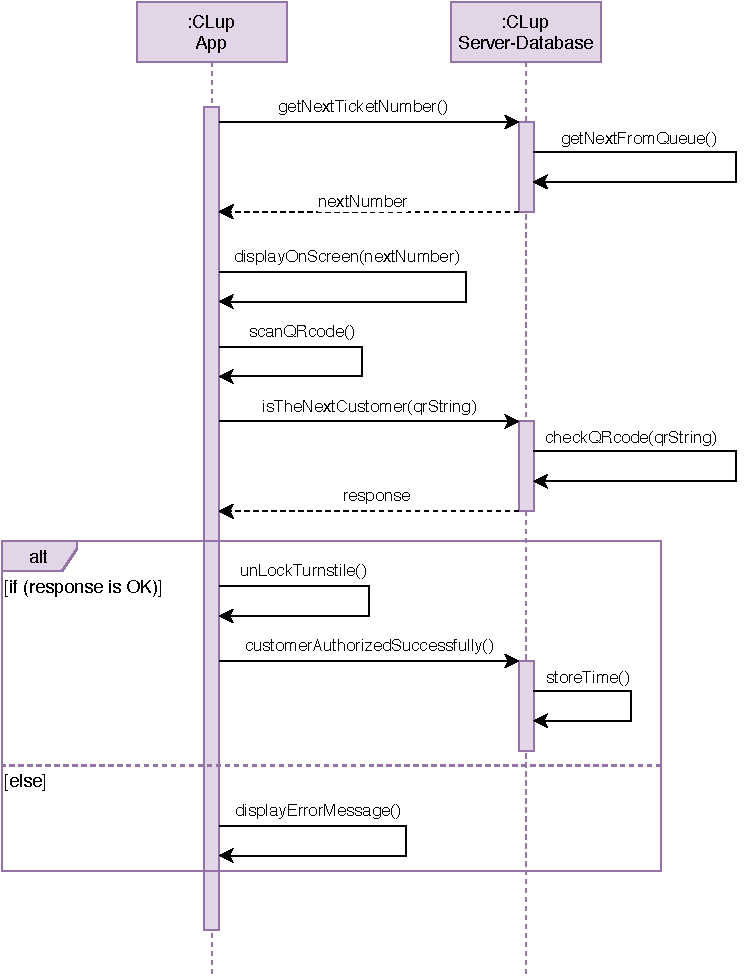
\includegraphics[width=1.0\textwidth]{images/authorizationToEnter_sequence_diagram.pdf}
	\caption{Sequence diagram reporting the activity periodically performed in background, by the application of the store manager, to authorize customers to enter in the store. For simplicity, the session authentication has been omitted.}
\end{figure}

\subsection{Mapping on Requirements}

\section{Performance Requirements}

\section{Design Constraints}

\subsection{Standard Compliance}
\subsection{Hardware limitations}
\subsection{Any Other Constraint}

\section{Software System Attributes}

\subsection{Reliability}
\subsection{Availability}
\subsection{Security}
\subsection{Maintainability}
\subsection{Portability}